\section{User Interface Design}
In this section, the user interface design will be presented using mockups within the short description.
The design focuses on optimizing the user experience and ensuring that the user can easily navigate on the website to perform the desired actions.
There will be separate in subsection to describe more clearly the main pages needed to satisfy the user requirements.

\subsection{Welcome Page}

\begin{figure}[H]
    \centering
    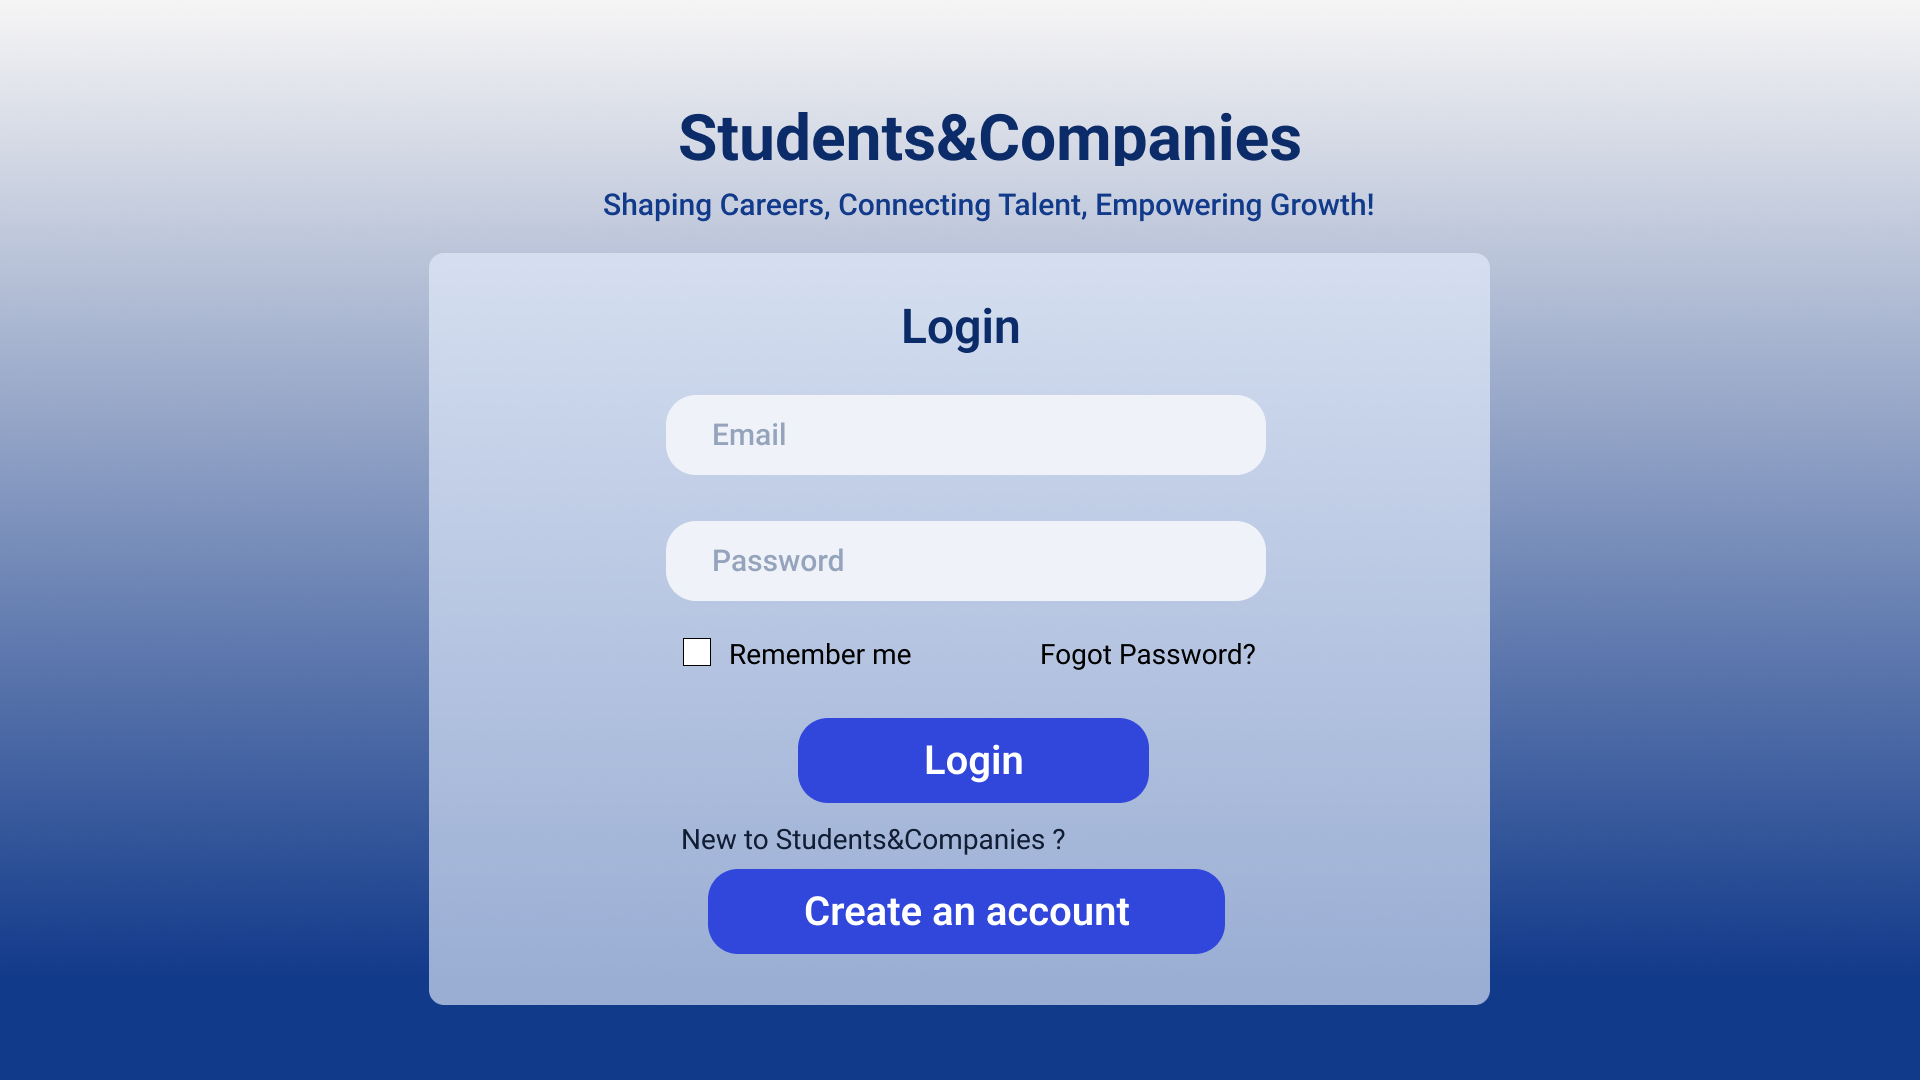
\includegraphics[width=0.8\textwidth]{Images/UI/Welcome Page.png}
    \caption{Welcome Page}\label{fig:Welcome_page}
\end{figure}

\subsection{Register Page}
If the User is not registered and wants to create an account, they will be asked to choose the type of account they want to create. 
Clicking on the type listed will redirect to the corresponding Register Page where the user can fill in the required information.
\begin{figure}[H]
    \centering
    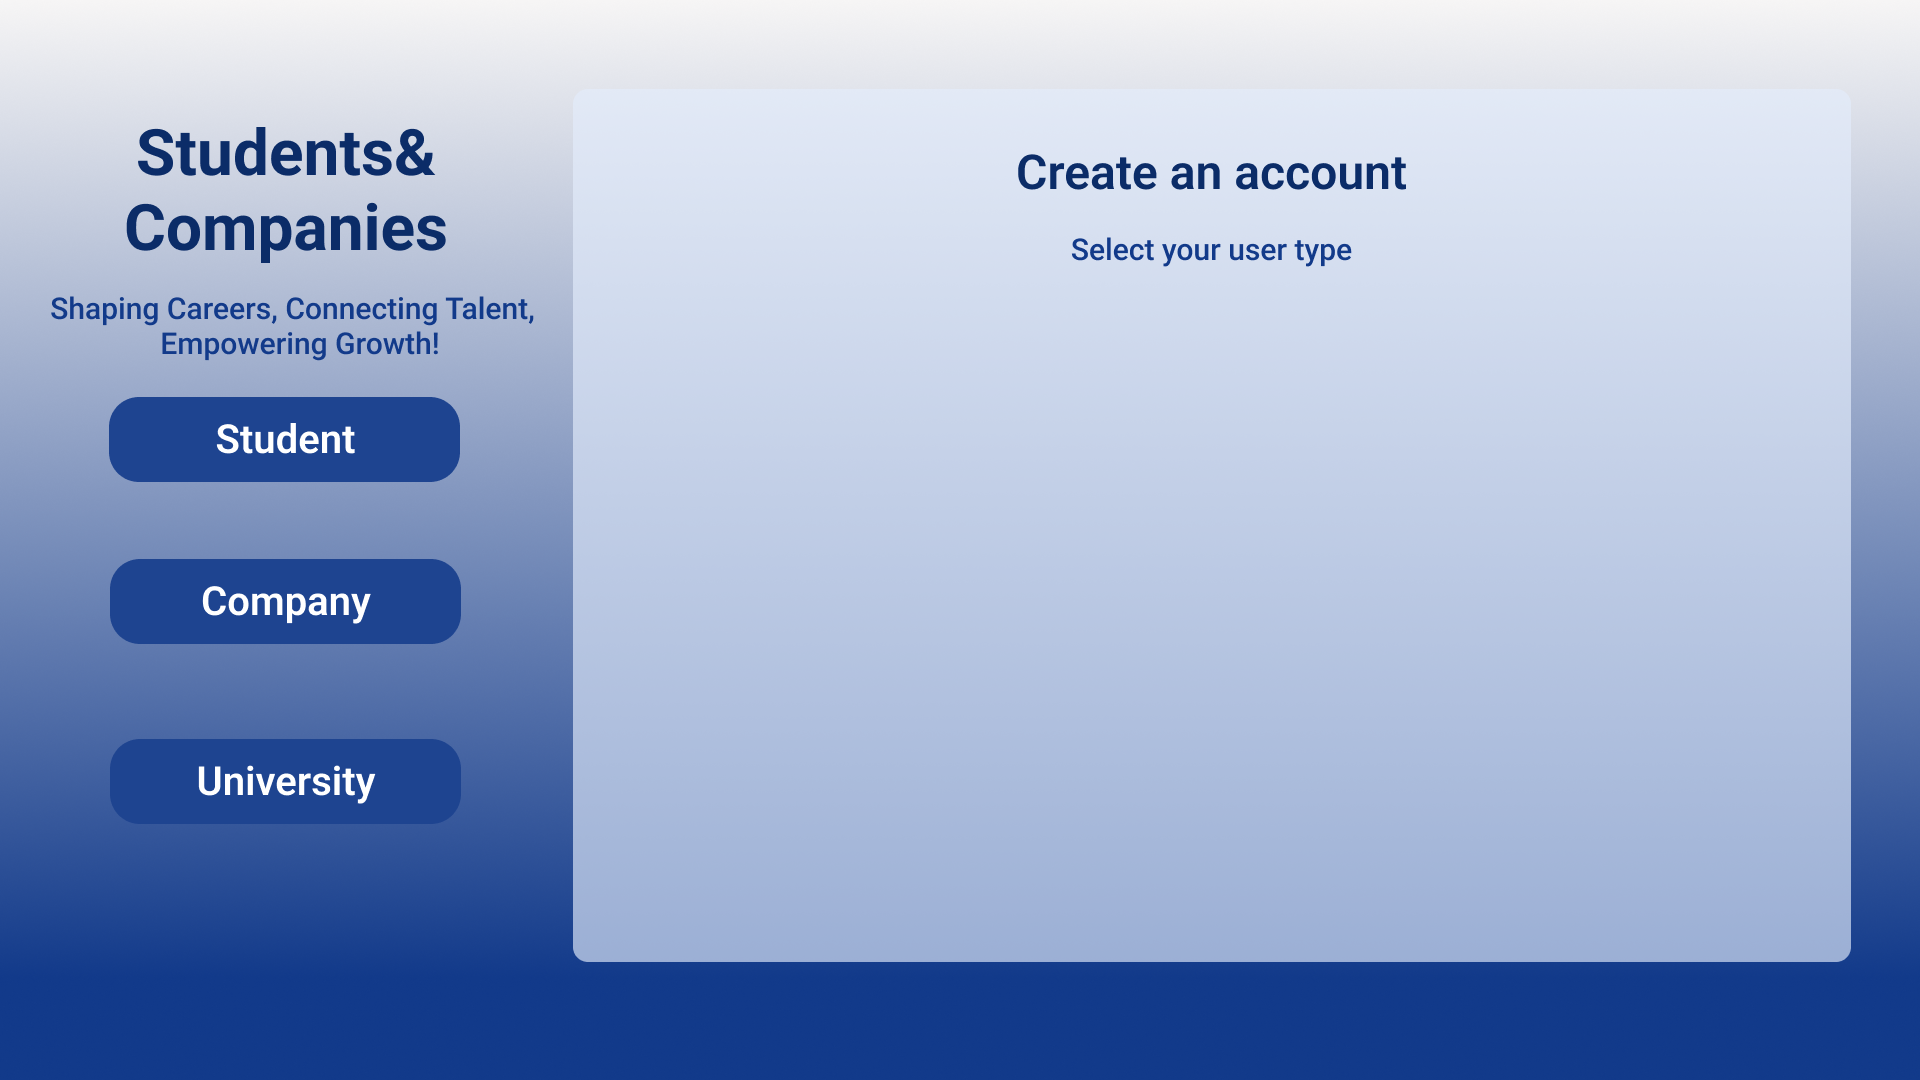
\includegraphics[width=0.8\textwidth]{Images/UI/Create account.png}
    \caption{Register Page}\label{fig:Creat_account}
\end{figure}

\begin{figure}[H]
    \centering
    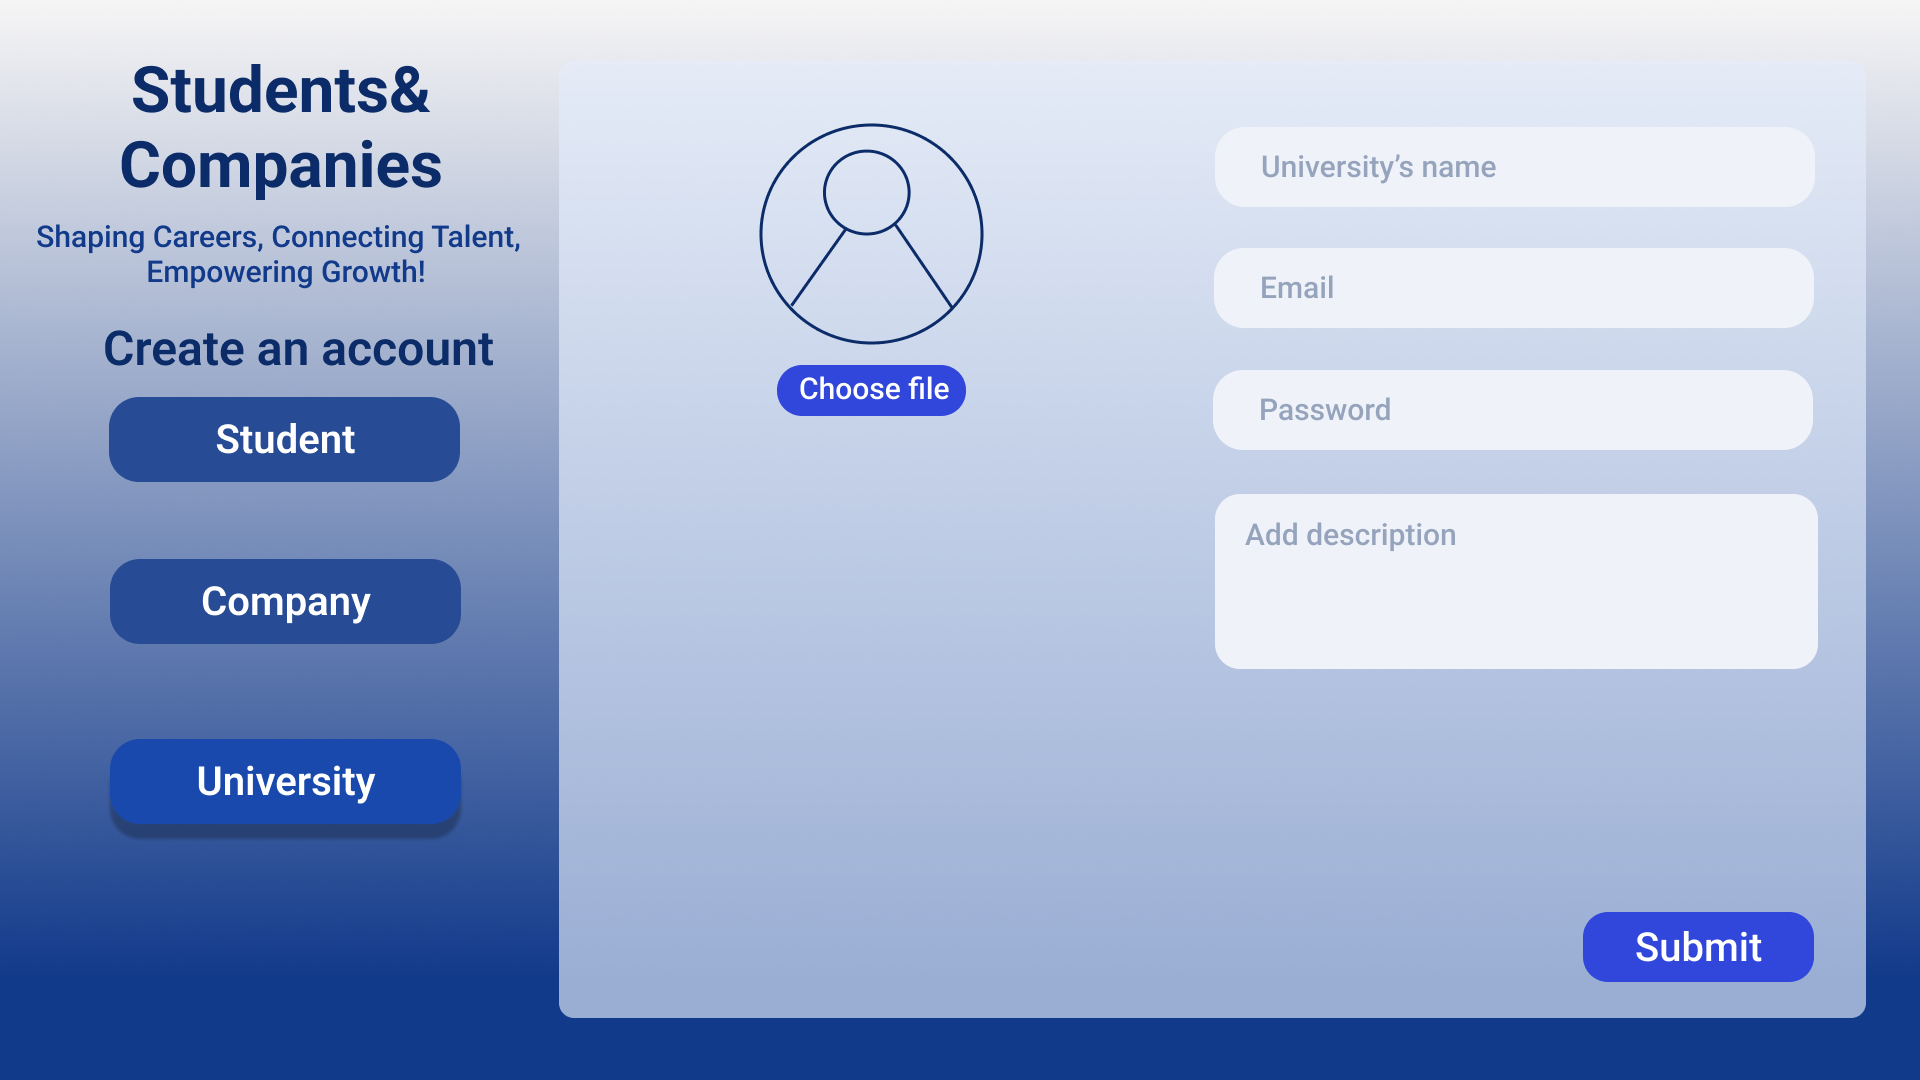
\includegraphics[width=0.8\textwidth]{Images/UI/Create account University.png}
    \caption{University create account}\label{fig:Creat_account University}
\end{figure}

\begin{figure}[H]
    \centering
    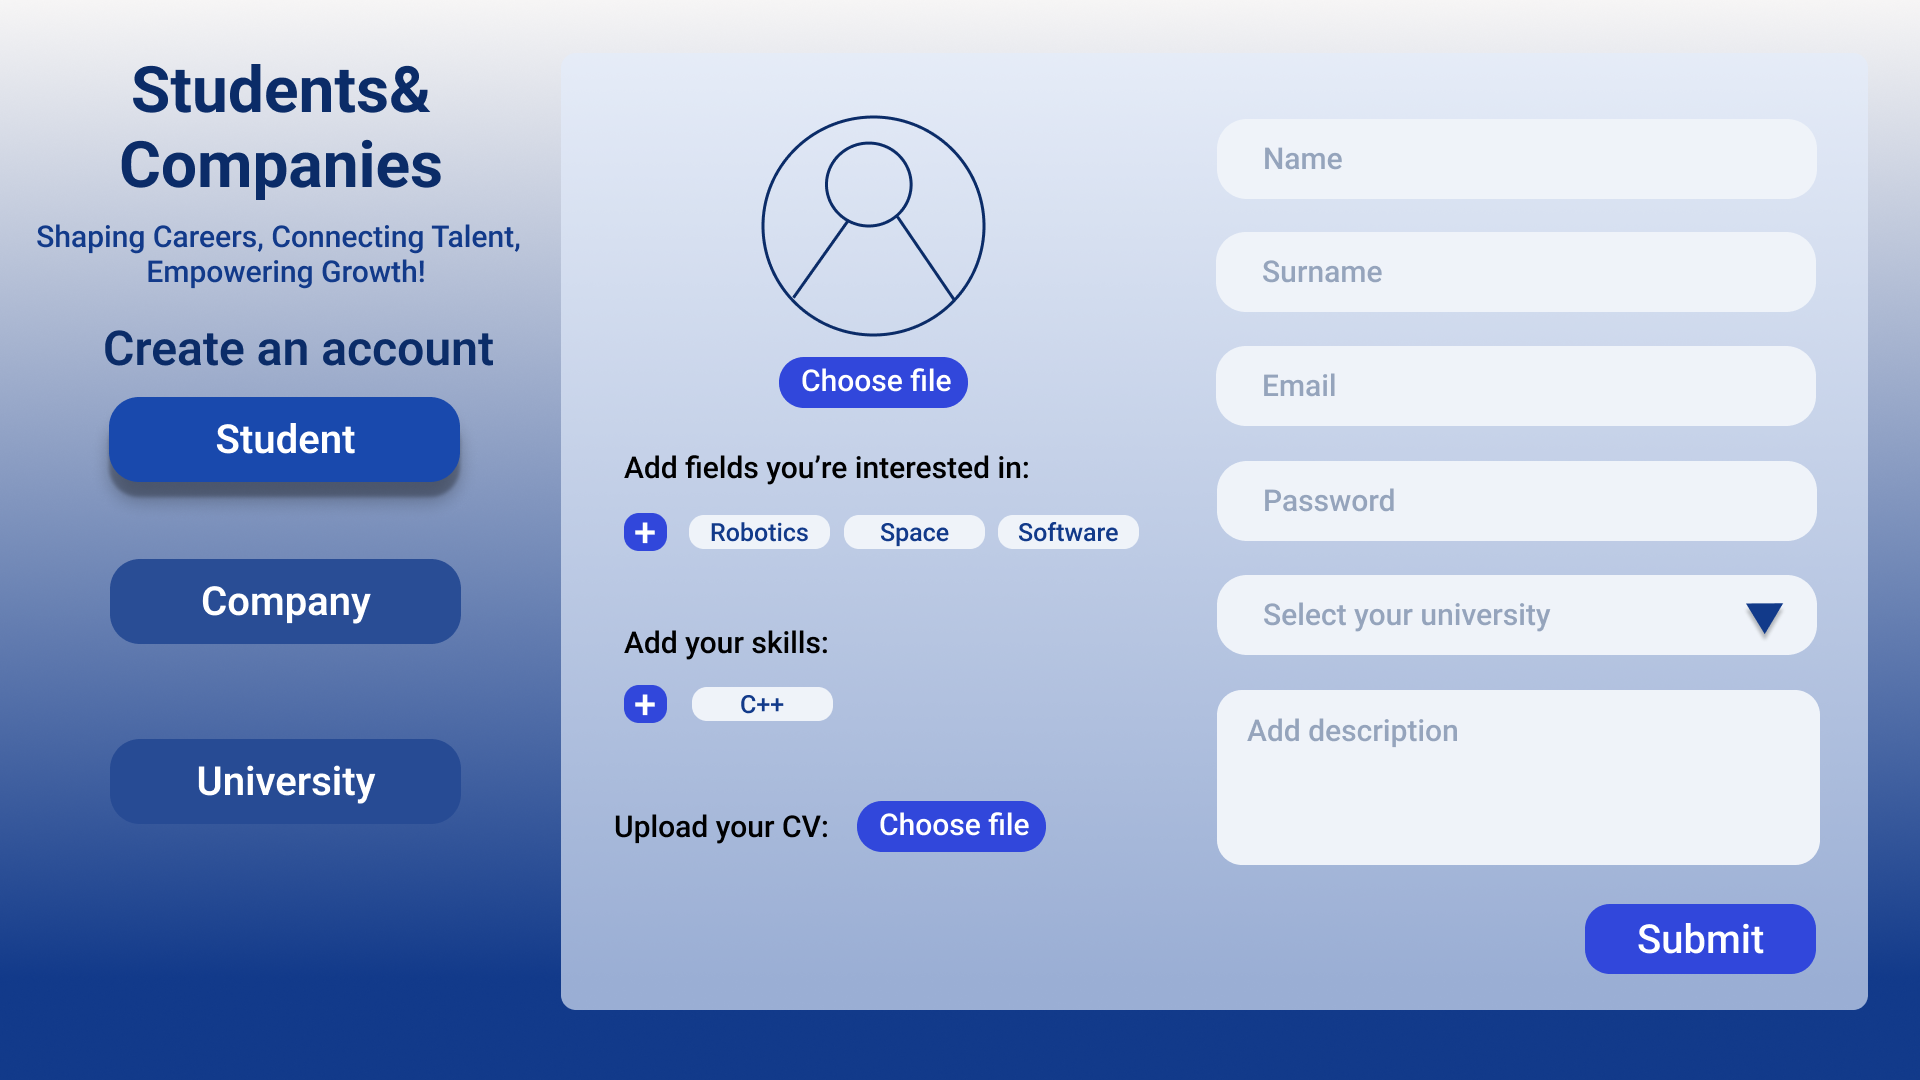
\includegraphics[width=0.8\textwidth]{Images/UI/Create account student.png}
    \caption{Student create account}\label{fig:Creat_account student}
\end{figure}

\begin{figure}[H]
    \centering
    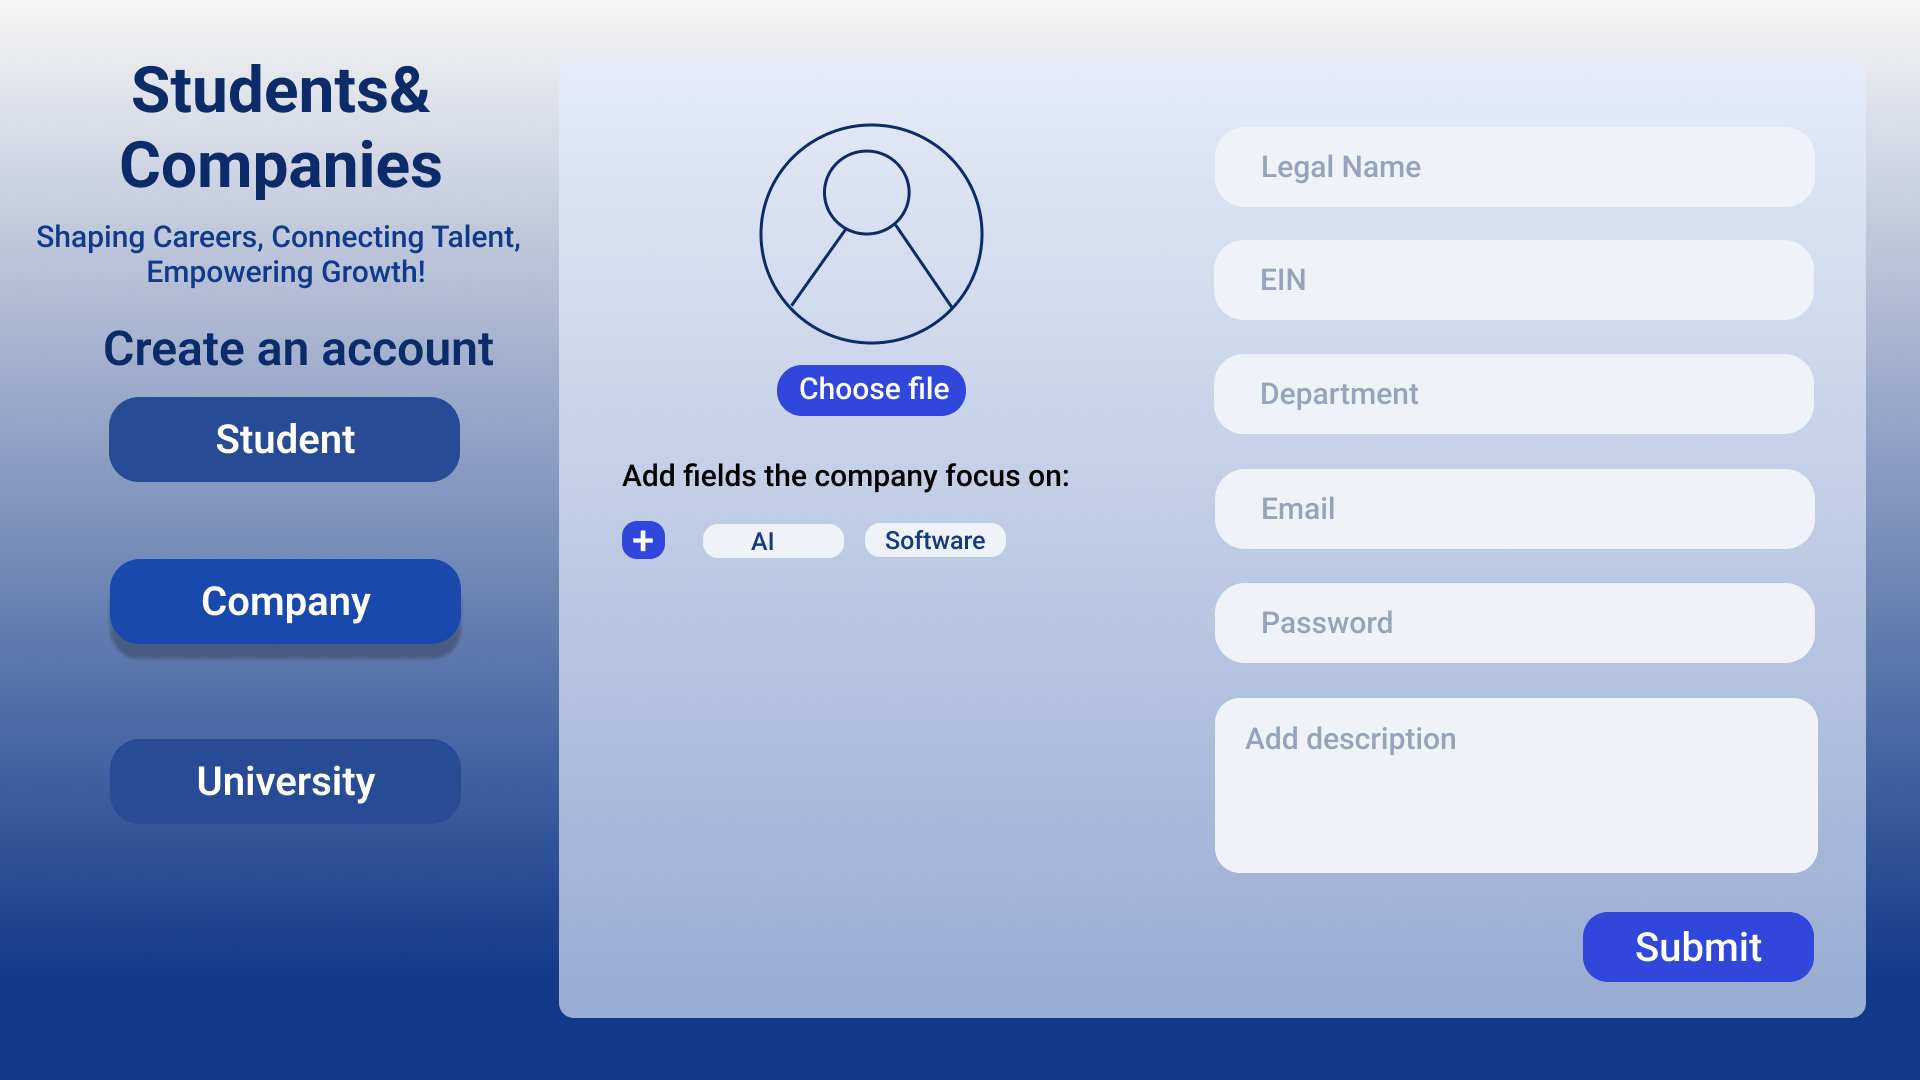
\includegraphics[width=0.8\textwidth]{Images/UI/Create account company.png}
    \caption{Company create account}\label{fig:Creat_account company}
\end{figure}
\subsection{Header bar}
The header bar is displayed on every page of the platform and contains the logo of the platform, 
the side menu button, the notification bell, and the user profile button. In particular, there 
is also the chat icon that allows the Student and Company to access available chat lists.

\subsection{Student's view}
Once access to the platform, to optimizing the user experience, the student will be able to use the side menu to navigate to the desired page:
\textit{Search, Dashboard, My applications and My internships}.
\begin{figure}[H]
    \centering
    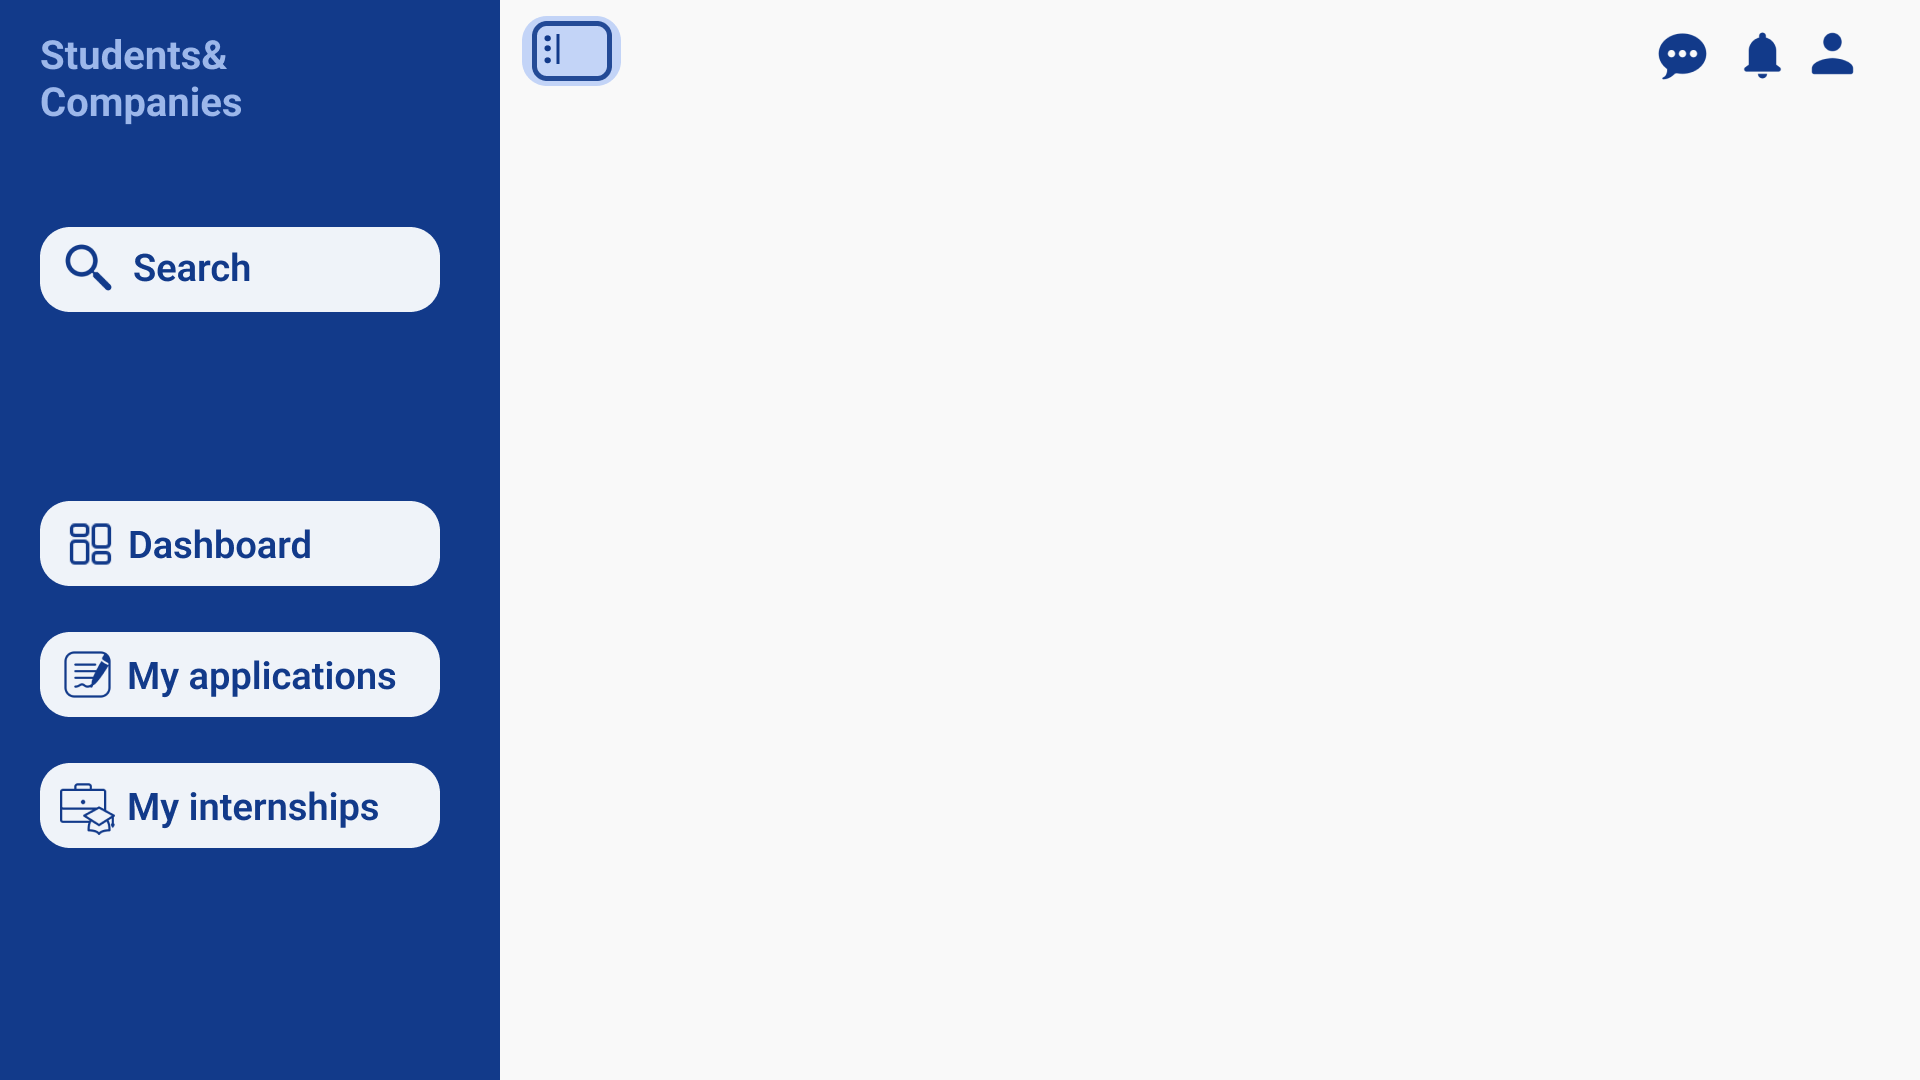
\includegraphics[width=0.8\textwidth]{Images/UI/Layout-Student.png}
    \caption{Student's Side Menu}\label{fig:Student_view}
\end{figure}
\subsubsection{Dashboard page}
By default, students are directed to the Dashboard page upon logging in.\\ 
The Dashboard provides an overview that allows students to quickly assess 
the current status of their applications and the performance of internships they are participating in or have completed.
Clicking on a specific application or internship within the overview list redirects students to a detailed page for that application or internship.\\
Next to the historical internship section, there is a window displaying the latest comments on the current internship with quick access to 
the Feedback and Complaint pages for the ongoing internship, click on \textit{Open}.\\
Additionally, students can use the search bar to find internships or user profiles by entering relevant keywords. Below the search bar, there is a
 \textit{Suggested Job Searches} section, where students can click on a keyword to quickly search for internships that match their interests.
Below this section, a list of recommended internship announcements tailored to the student is displayed. Each announcement includes a brief description, 
and students can take one of three actions:
\begin{itemize}
    \item[-] Click the \textit{Apply Now} button to apply for the internship.
    \item[-] Click the block to view more details about the internship announcement.
    \item[-] Click the \textit{X} to remove the internship announcement from the display.
\end{itemize}
\begin{figure}[H]
    \centering
    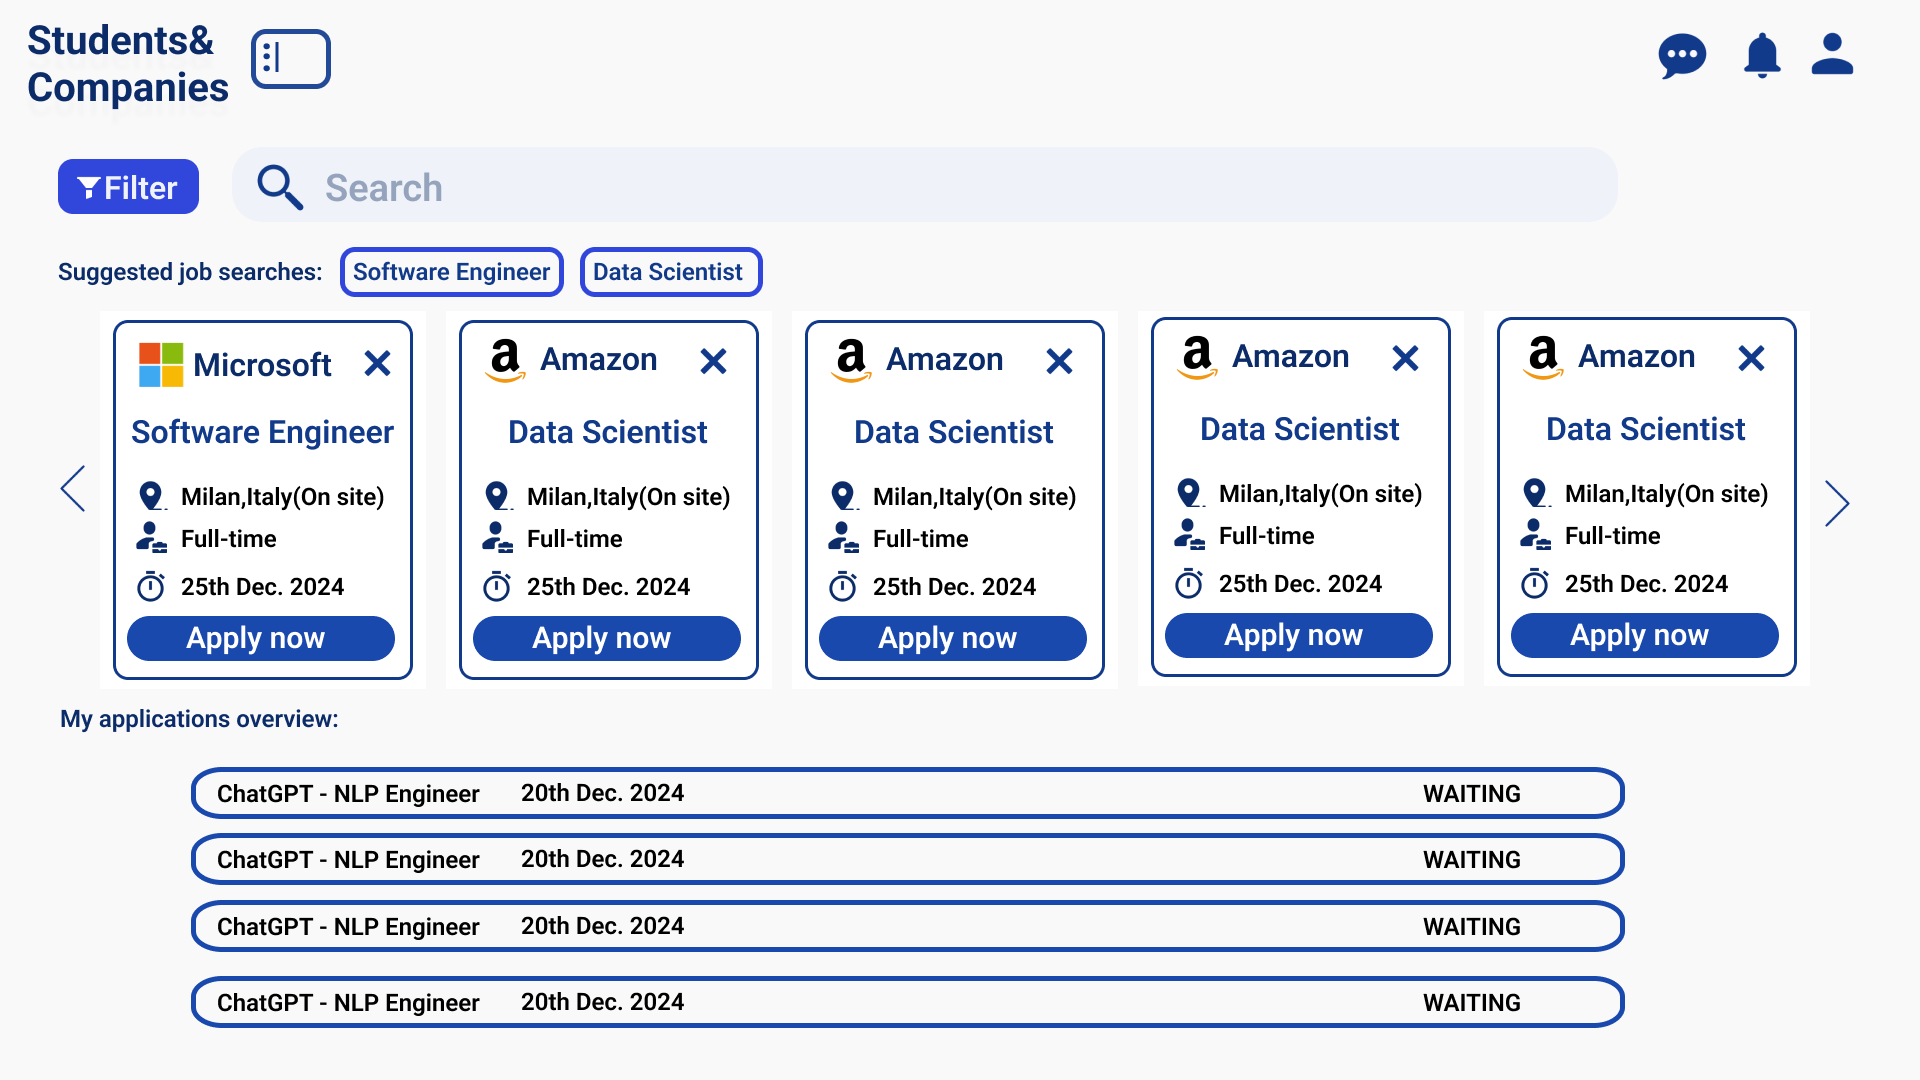
\includegraphics[width=0.8\textwidth]{Images/UI/Dashboard 1-student.png}
    \caption{Student's Dashboard 1}\label{fig:DashboardStudent1}
\end{figure}

\begin{figure}[H]
    \centering
    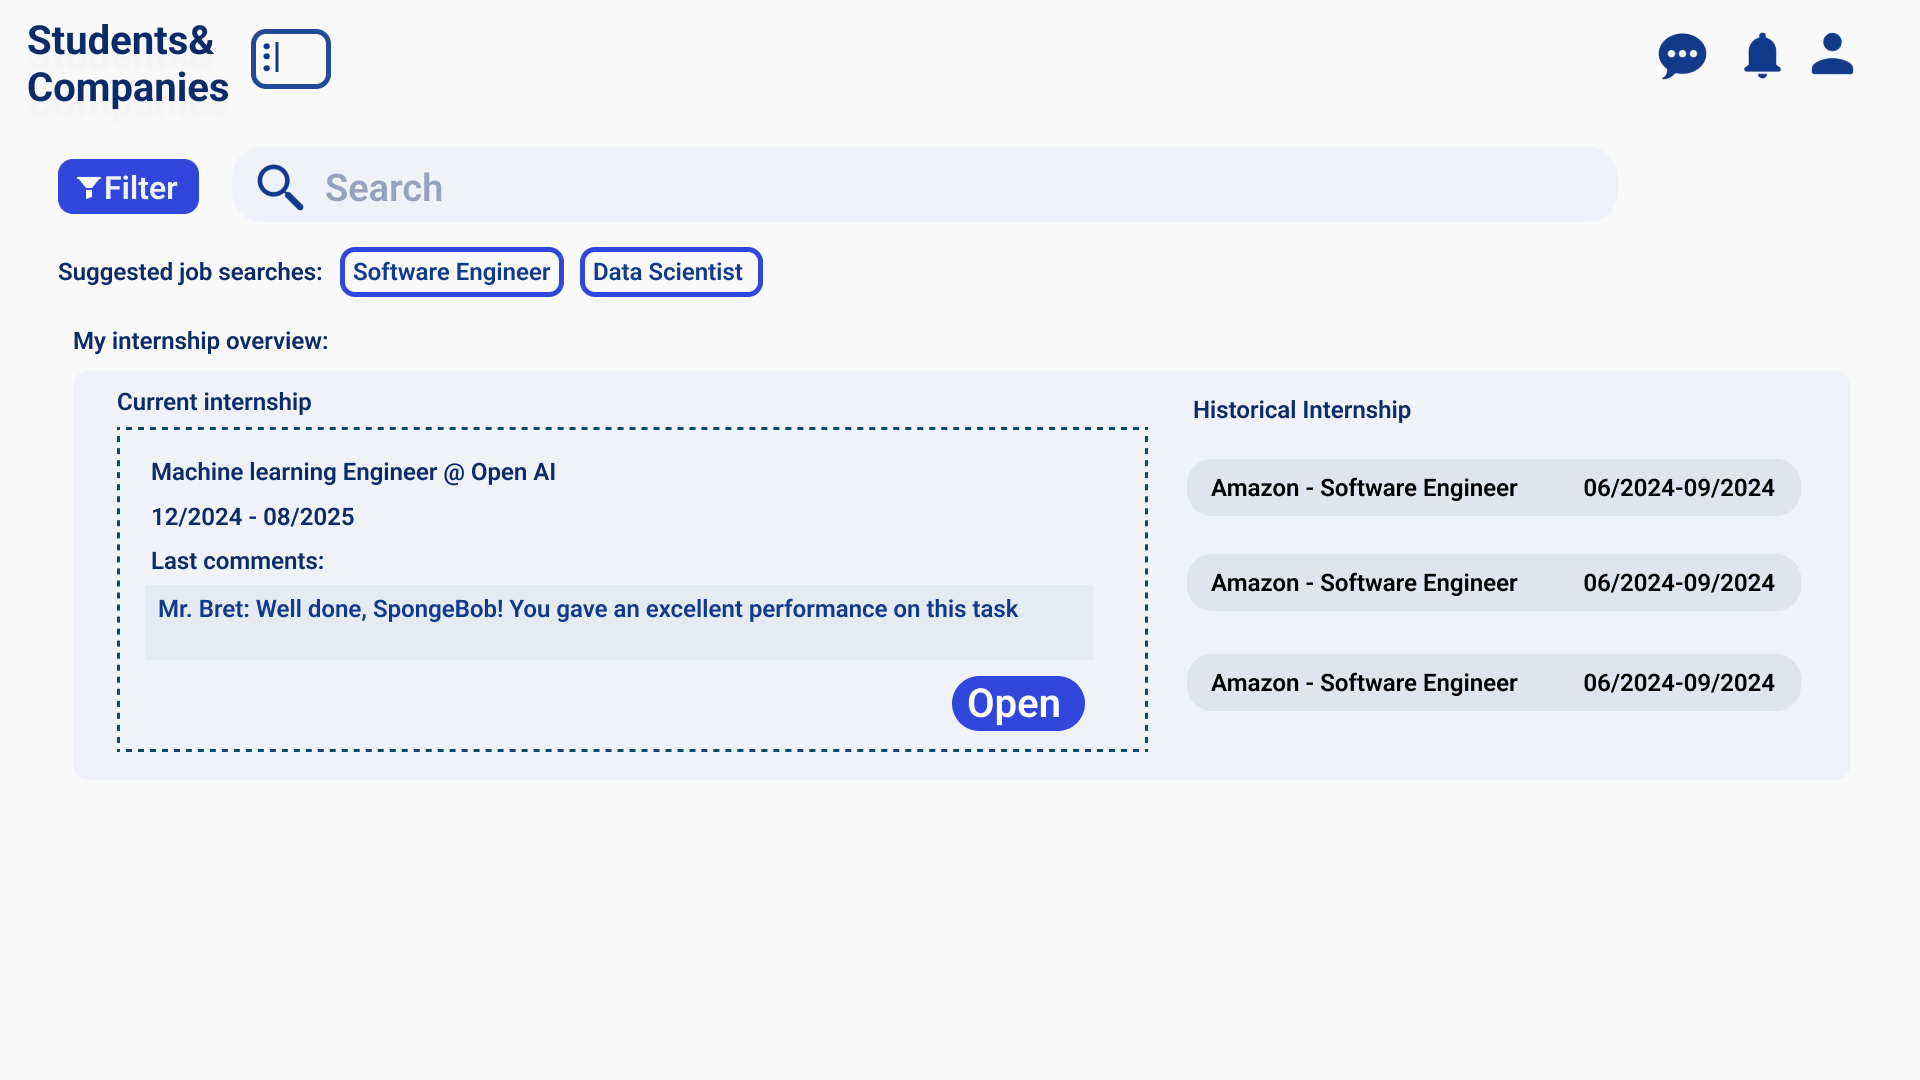
\includegraphics[width=0.8\textwidth]{Images/UI/Dashboard 2-student.png}
    \caption{Student's Dashboard 2}\label{fig:Dashboard Student 2}
\end{figure}
\subsubsection{My application page}
Here in figure\ref{fig:My application}, the student can view the status of their applications and take action based on the status of the application:
\begin{itemize}
    \item[-] Click on the \textit{View details} button to view the page with details of the internship announcement, figure\ref{fig:Internship announcement details}.
    \item[-] Click on the \textit{Invited to interview} button to view the details of the interview and questionnaire requested by the company to fill in, figure\ref{fig:Interview details 1}.
    \item[-] Click on the \textit{Accept or Reject Offer} button to view the details offer letter and to take the decision to accept or reject the offer, figure\ref{fig:Accept or Reject Offer}.
\end{itemize}
\begin{figure}[H]
    \centering
    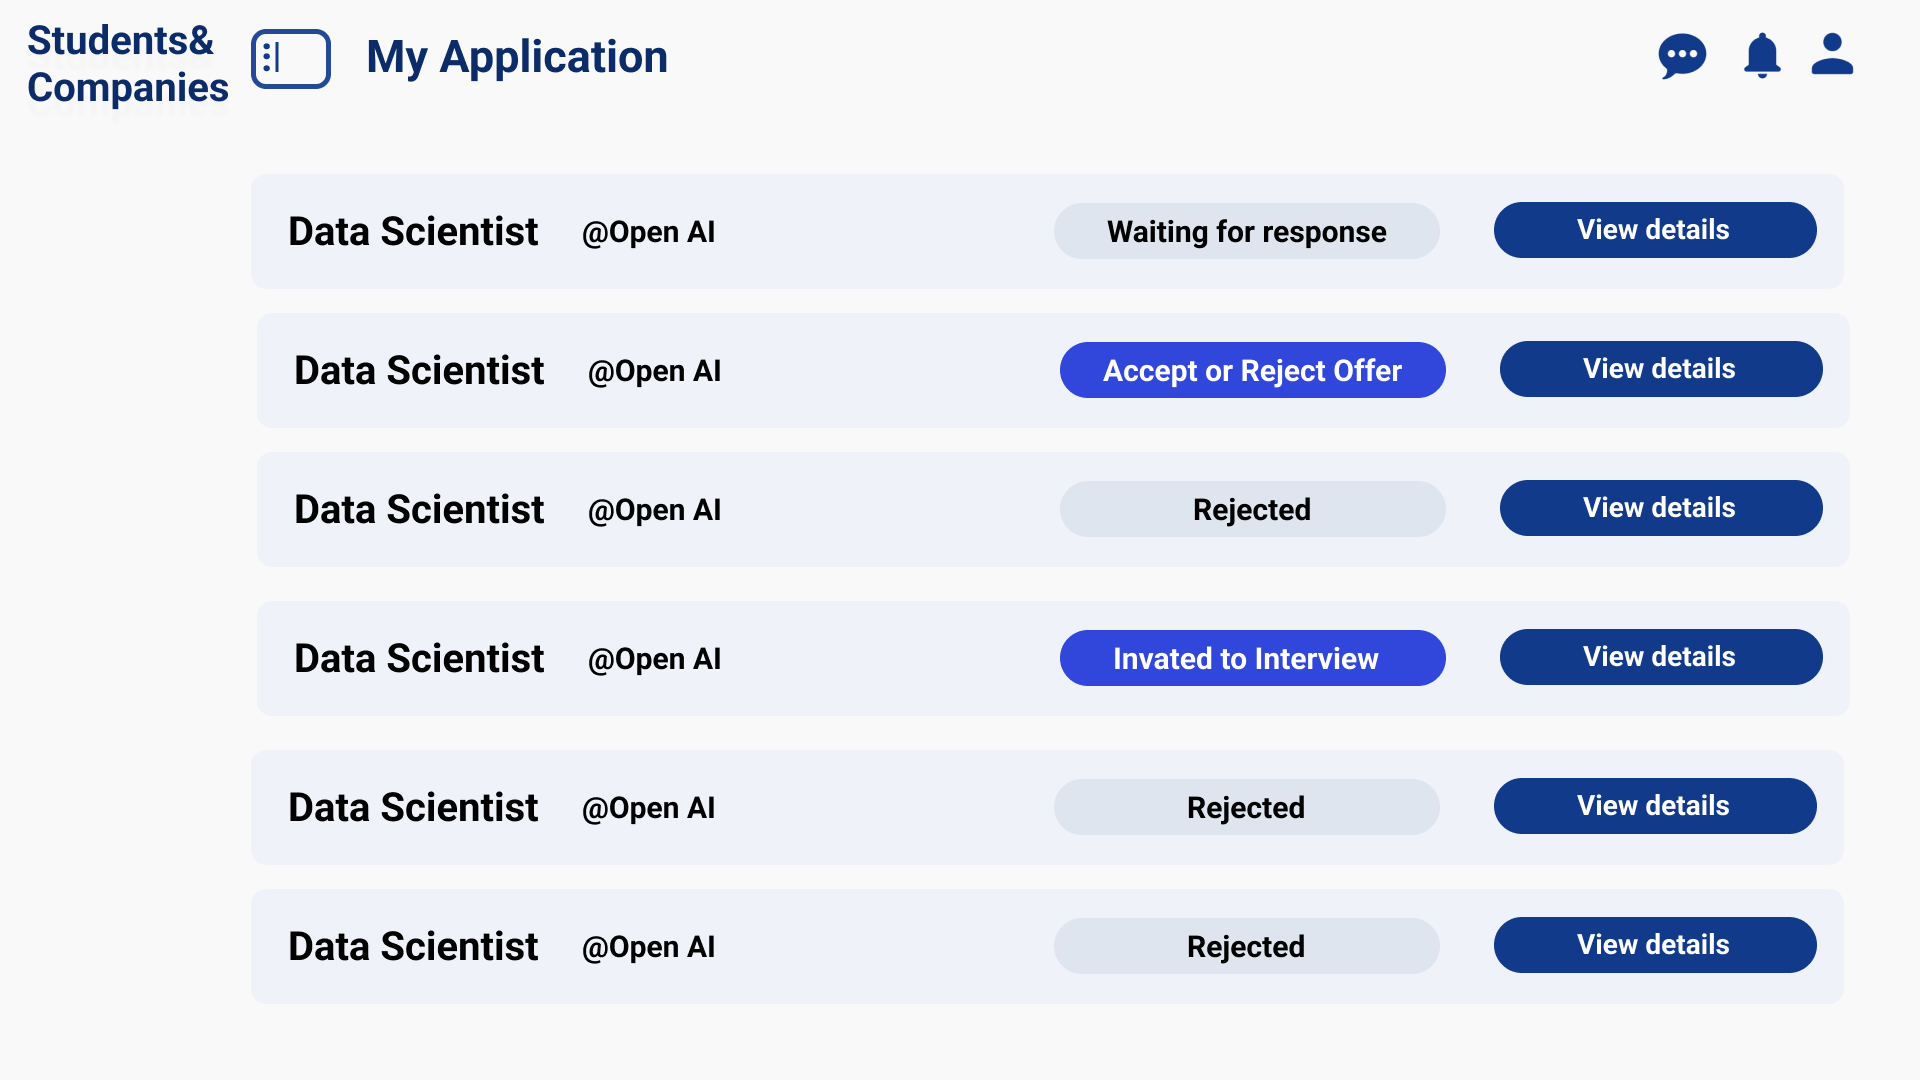
\includegraphics[width=0.8\textwidth]{Images/UI/My Application-student.png}
    \caption{My application}\label{fig:My application}
\end{figure}
\subsubsection{Interview details page}
Show the detail information related to the interview and the pre-interview questionnaire asked by the company to candidate to fill in.\\
Once completed all questions with the provided answers, the student can click on the \textit{Submit} button to send the answers to the company and save the answers in the platform for future reference.
\begin{figure}[H]
    \centering
    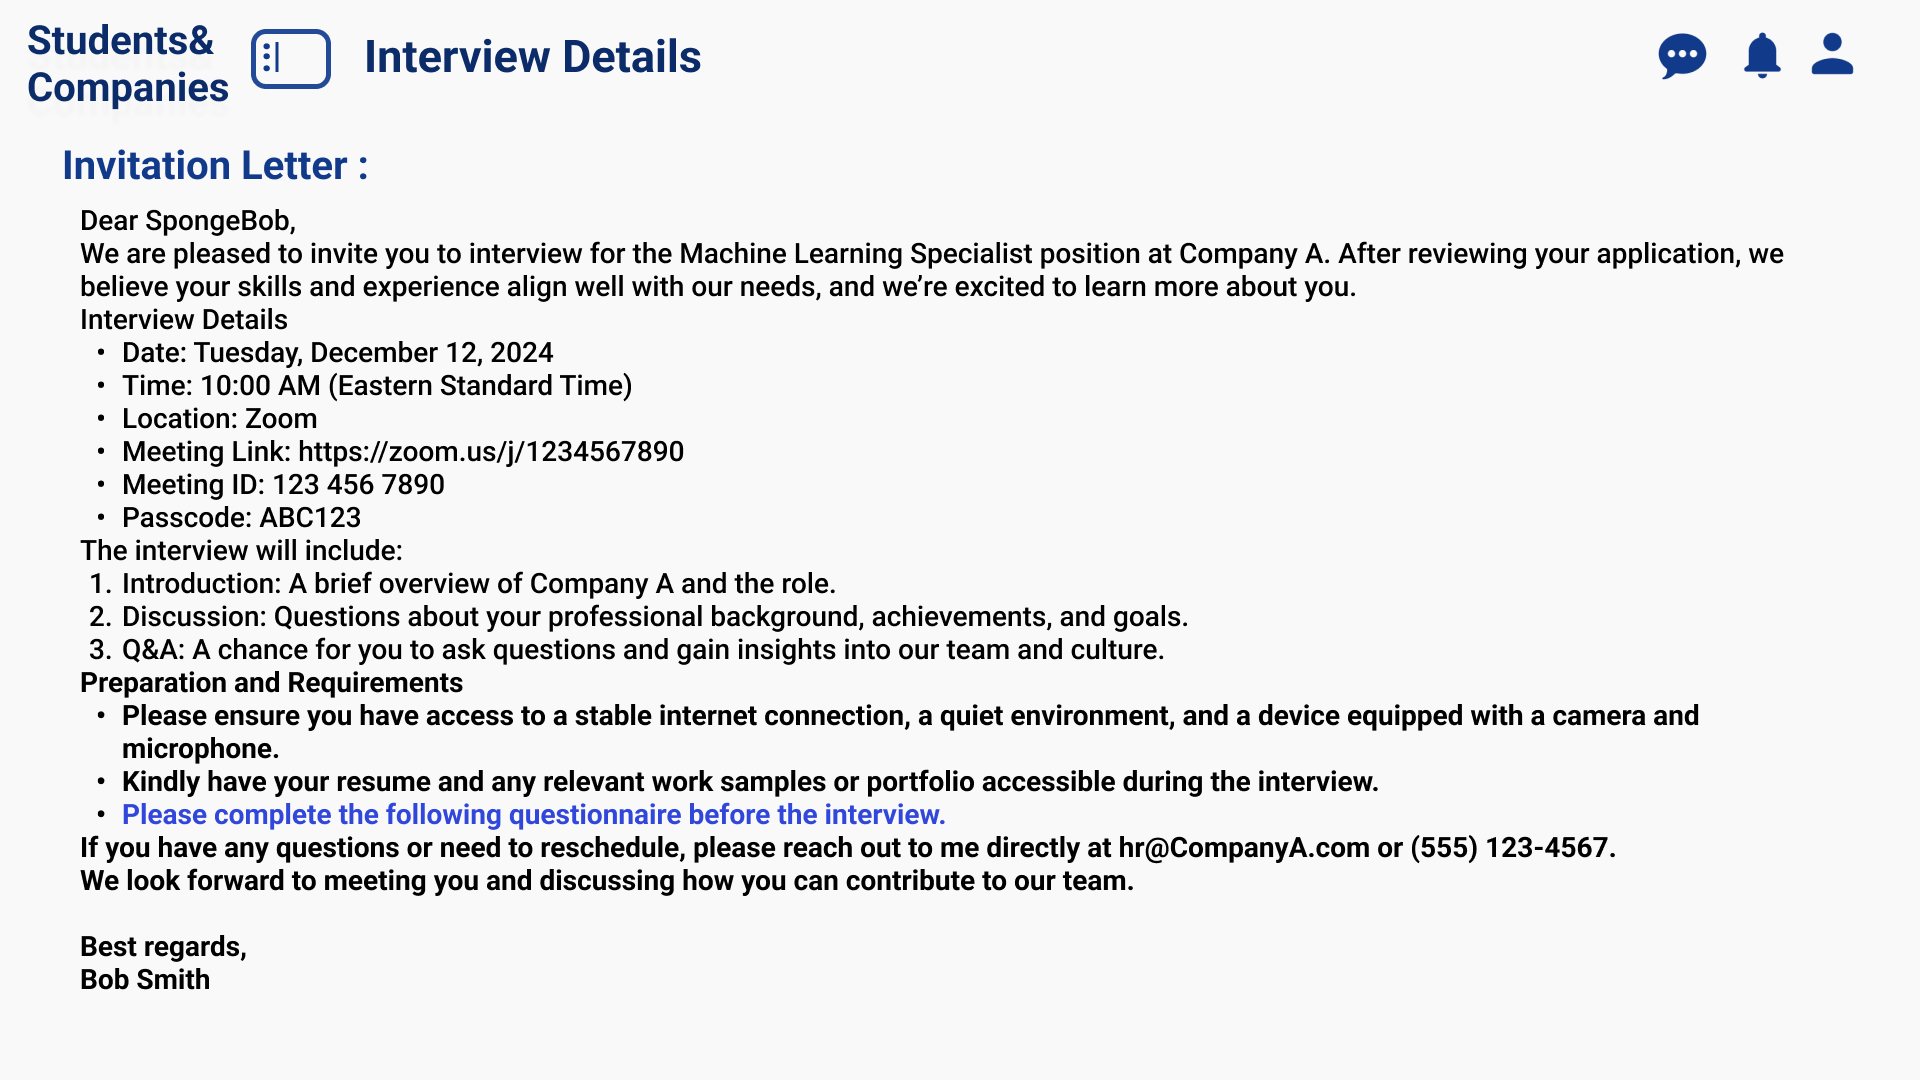
\includegraphics[width=0.8\textwidth]{Images/UI/Interview Details-student.png}
    \caption{Interview details 1}\label{fig:Interview details 1}
\end{figure}

\begin{figure}[H]
    \centering
    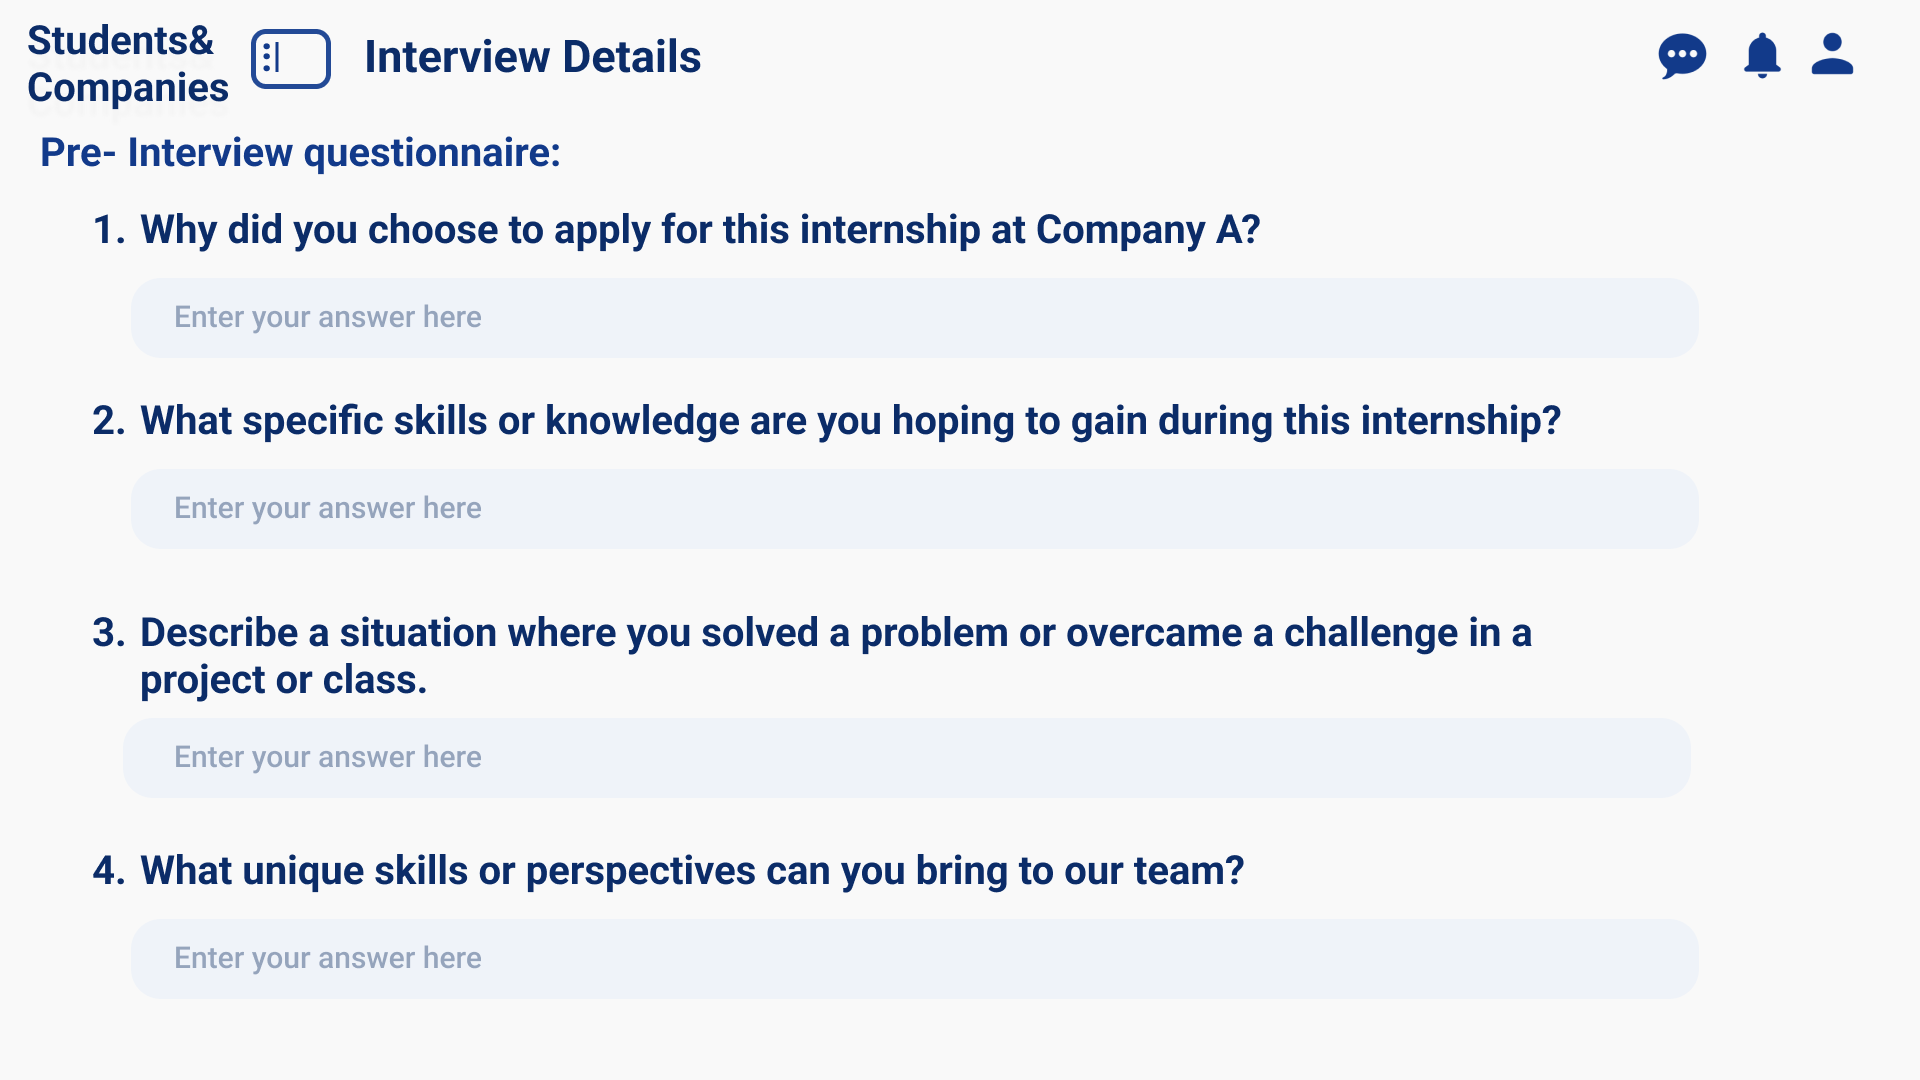
\includegraphics[width=0.8\textwidth]{Images/UI/Interview Details2-student.png}
    \caption{Interview details 2}\label{fig:Interview details 2}
\end{figure}

\begin{figure}[H]
    \centering
    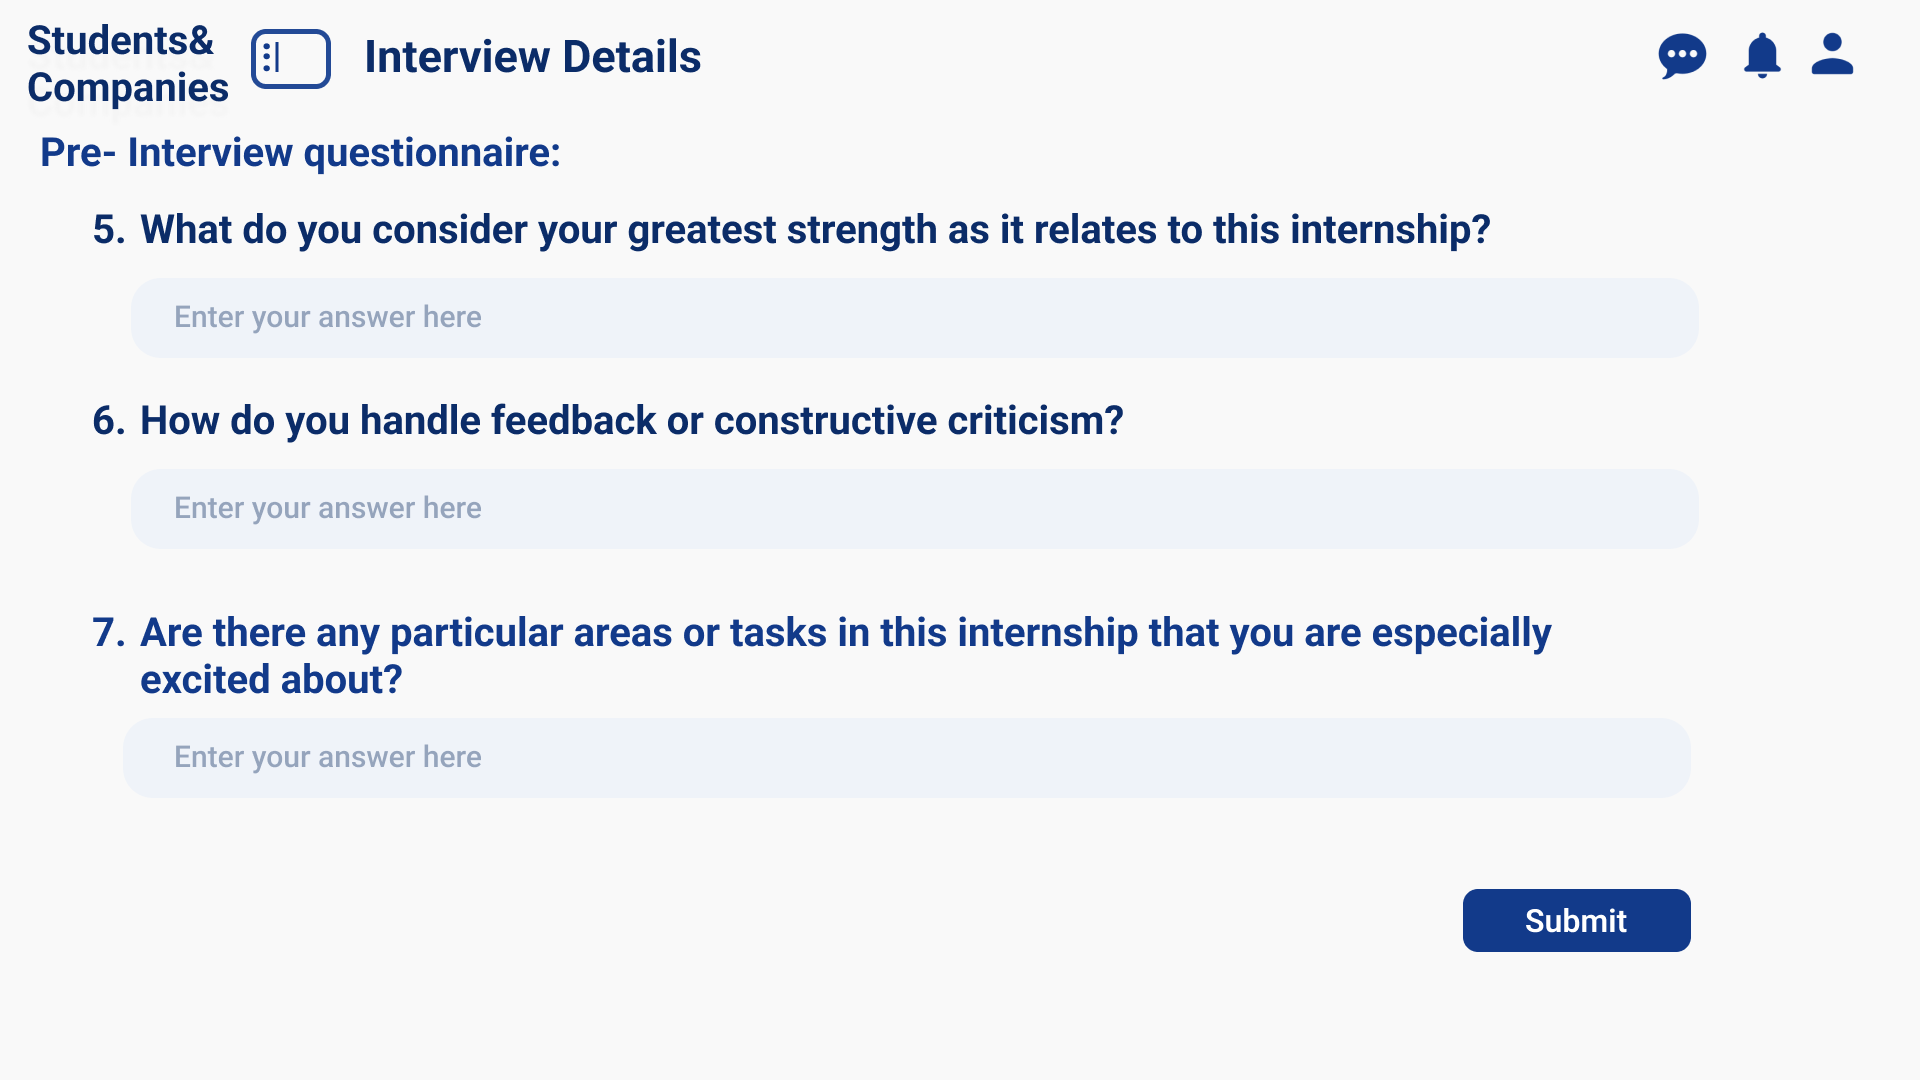
\includegraphics[width=0.8\textwidth]{Images/UI/Interview Details3-student.png}
    \caption{Interview details 3}\label{fig:Interview details 3}
\end{figure}
\subsubsection{Offer page}
Provide the offer letter sent by the company to the student. The student can take the decision to accept or reject the offer by clicking on the corresponding button.
Then the student decision will be sent to the company and recorded in the database, the application status will be updated accordingly.
\begin{figure}[H]
    \centering
    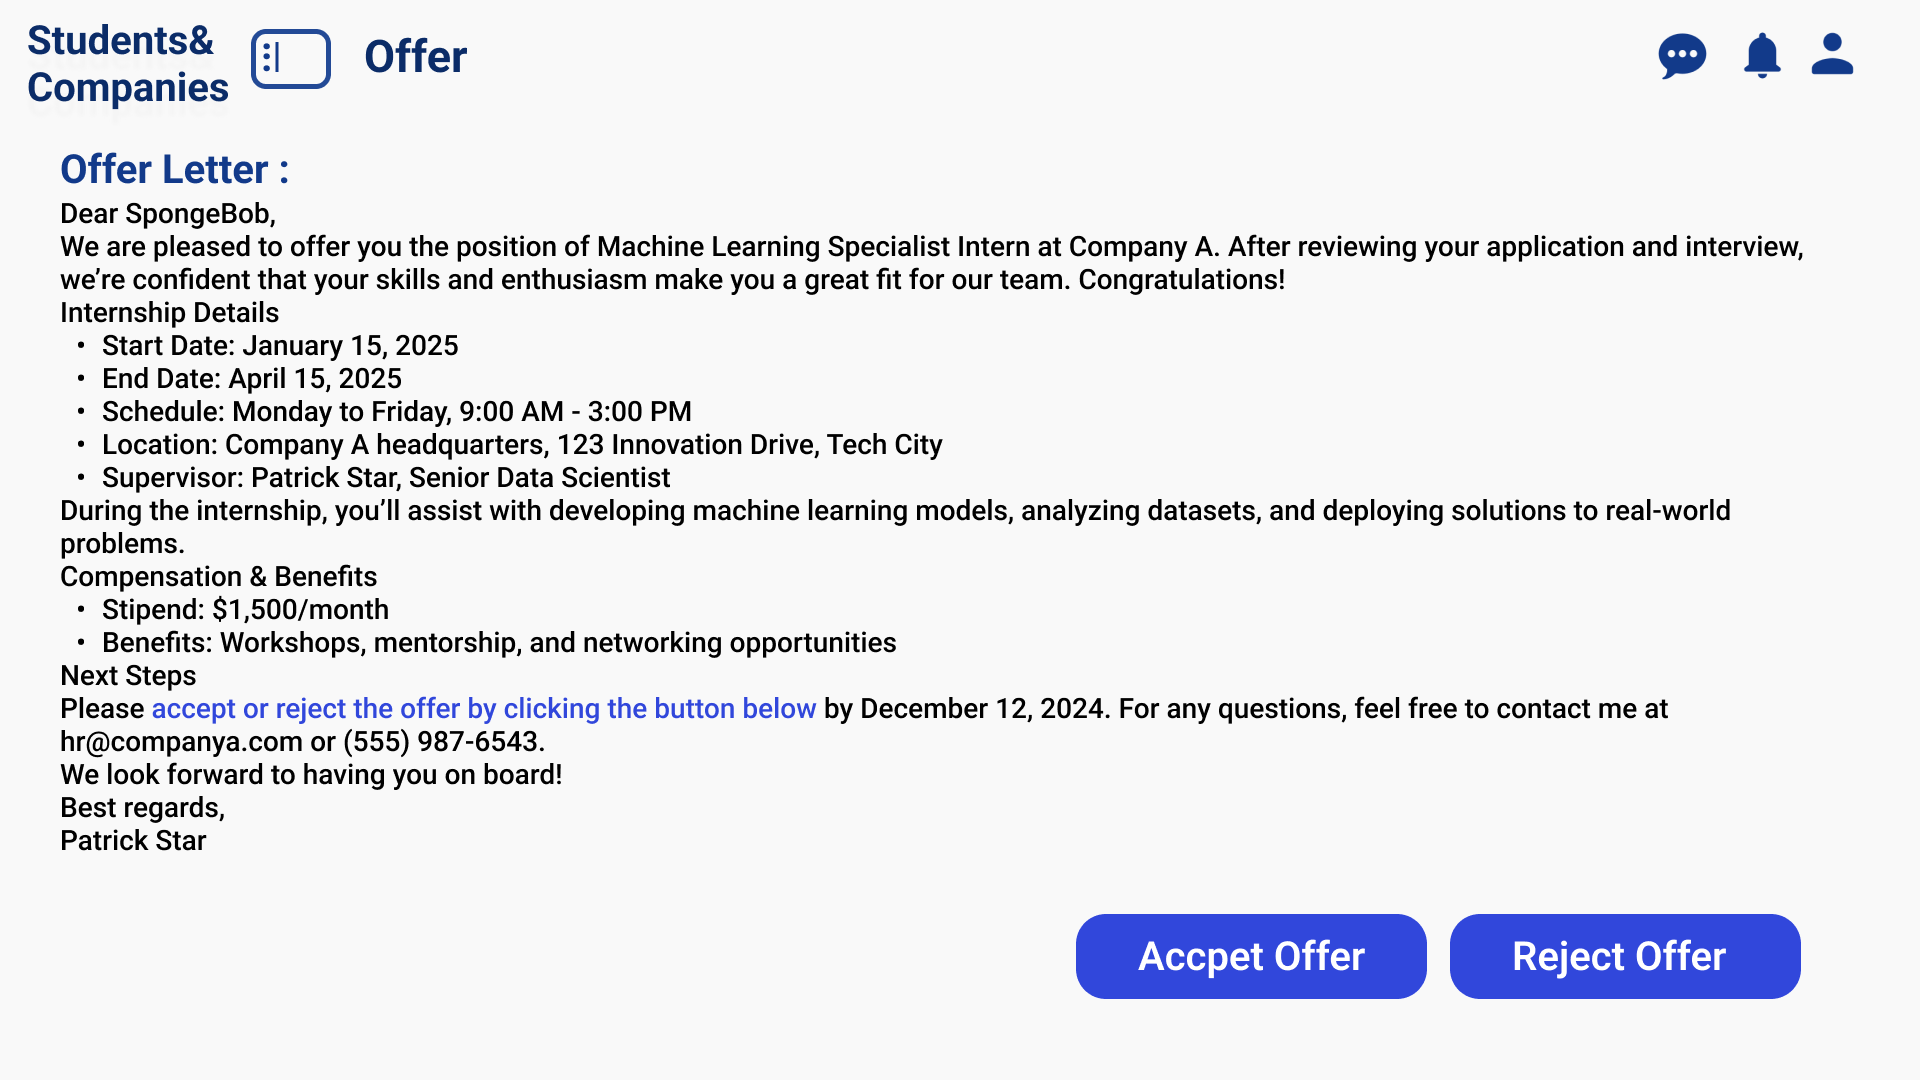
\includegraphics[width=0.8\textwidth]{Images/UI/Reject-student.png}
    \caption{Accept or Reject Offer }\label{fig:Accept or Reject Offer}
\end{figure}
\subsubsection{My internship page}
Here in figure\ref{fig:My internship}, the student can view the list of internships they are participating in or have completed.\\
For the current internship, the student can access the feedback and complaint page by clicking on the \textit{Add comments} button. \\
For the historical internship, the student can view the feedback and complaints recorded by the company and the student during the internship clicking
on the \textit{View details} button.
\begin{figure}[H]
    \centering
    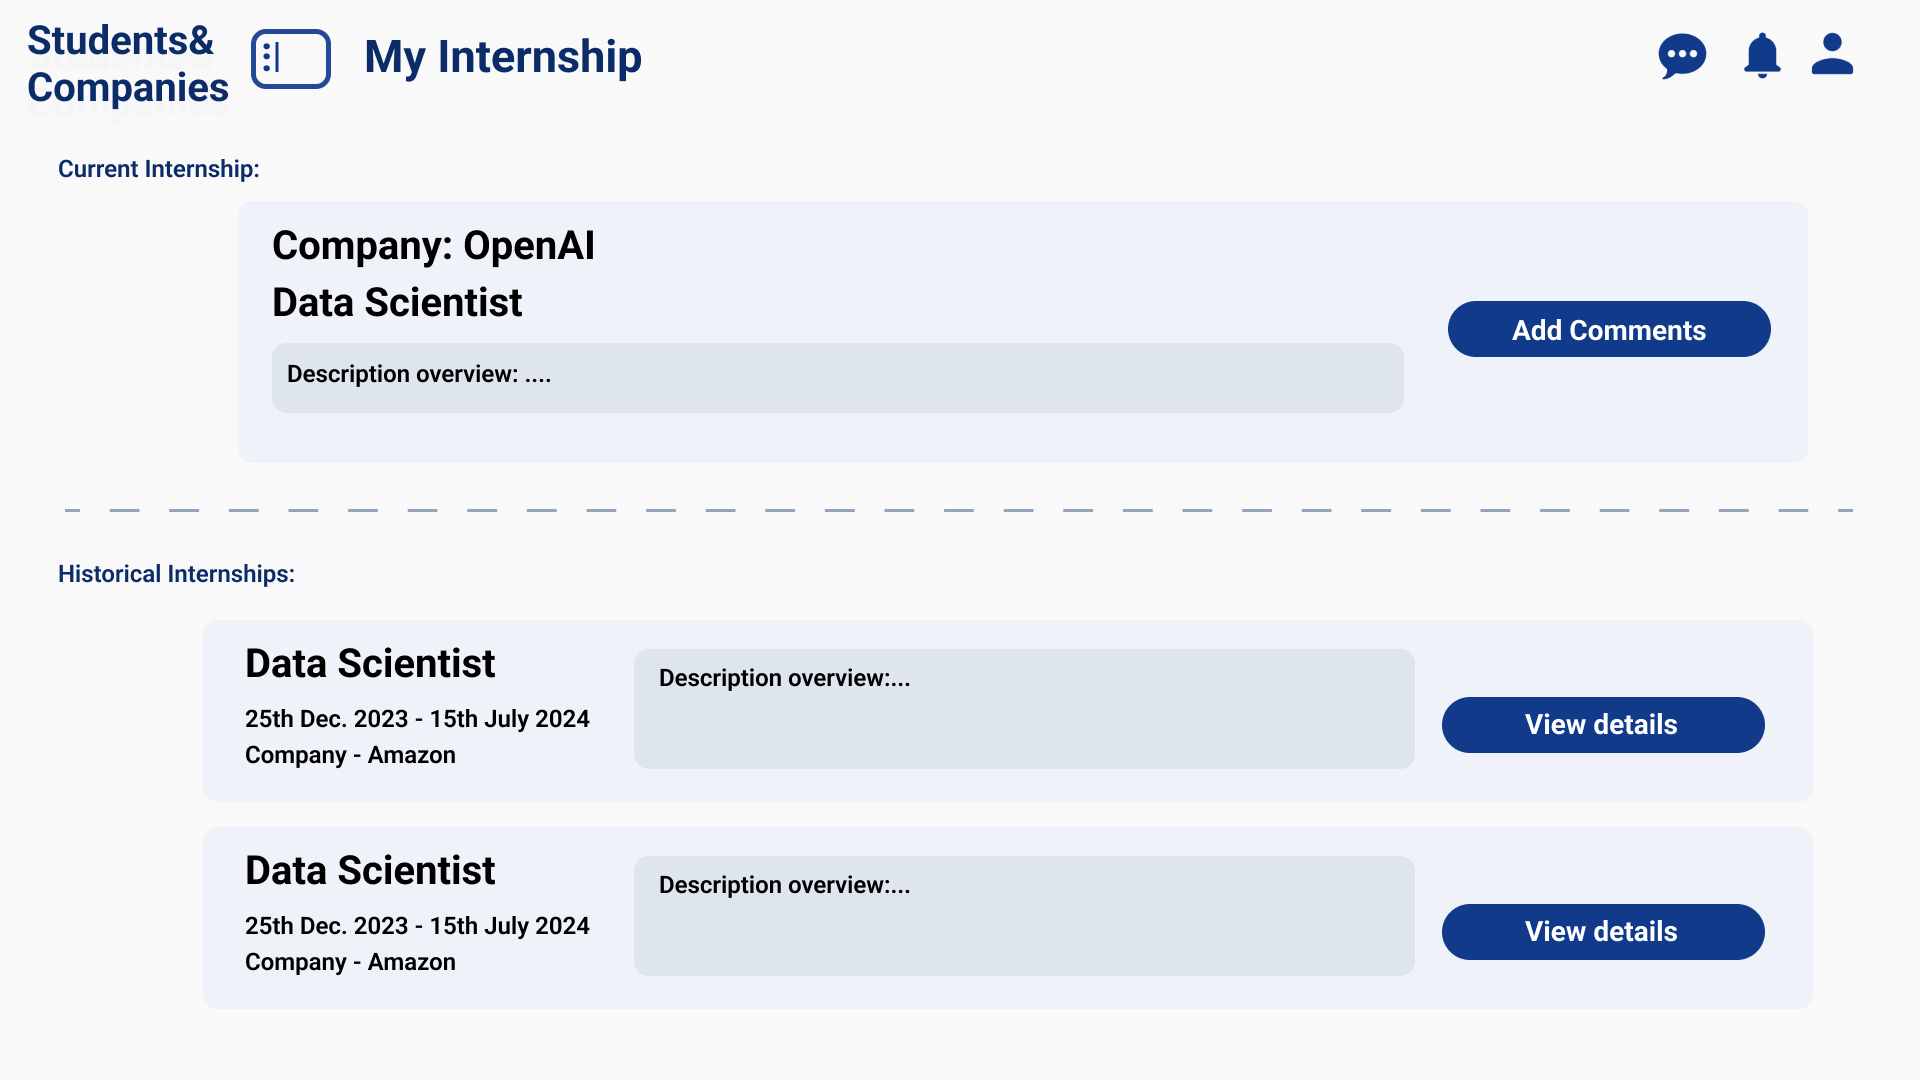
\includegraphics[width=0.8\textwidth]{Images/UI/My Internship-student.png}
    \caption{My internship }\label{fig:My internship}
\end{figure}
\subsubsection{Internship announcement page}
Represents the internship announcement details by the student's view side.
\begin{figure}[H]
    \centering
    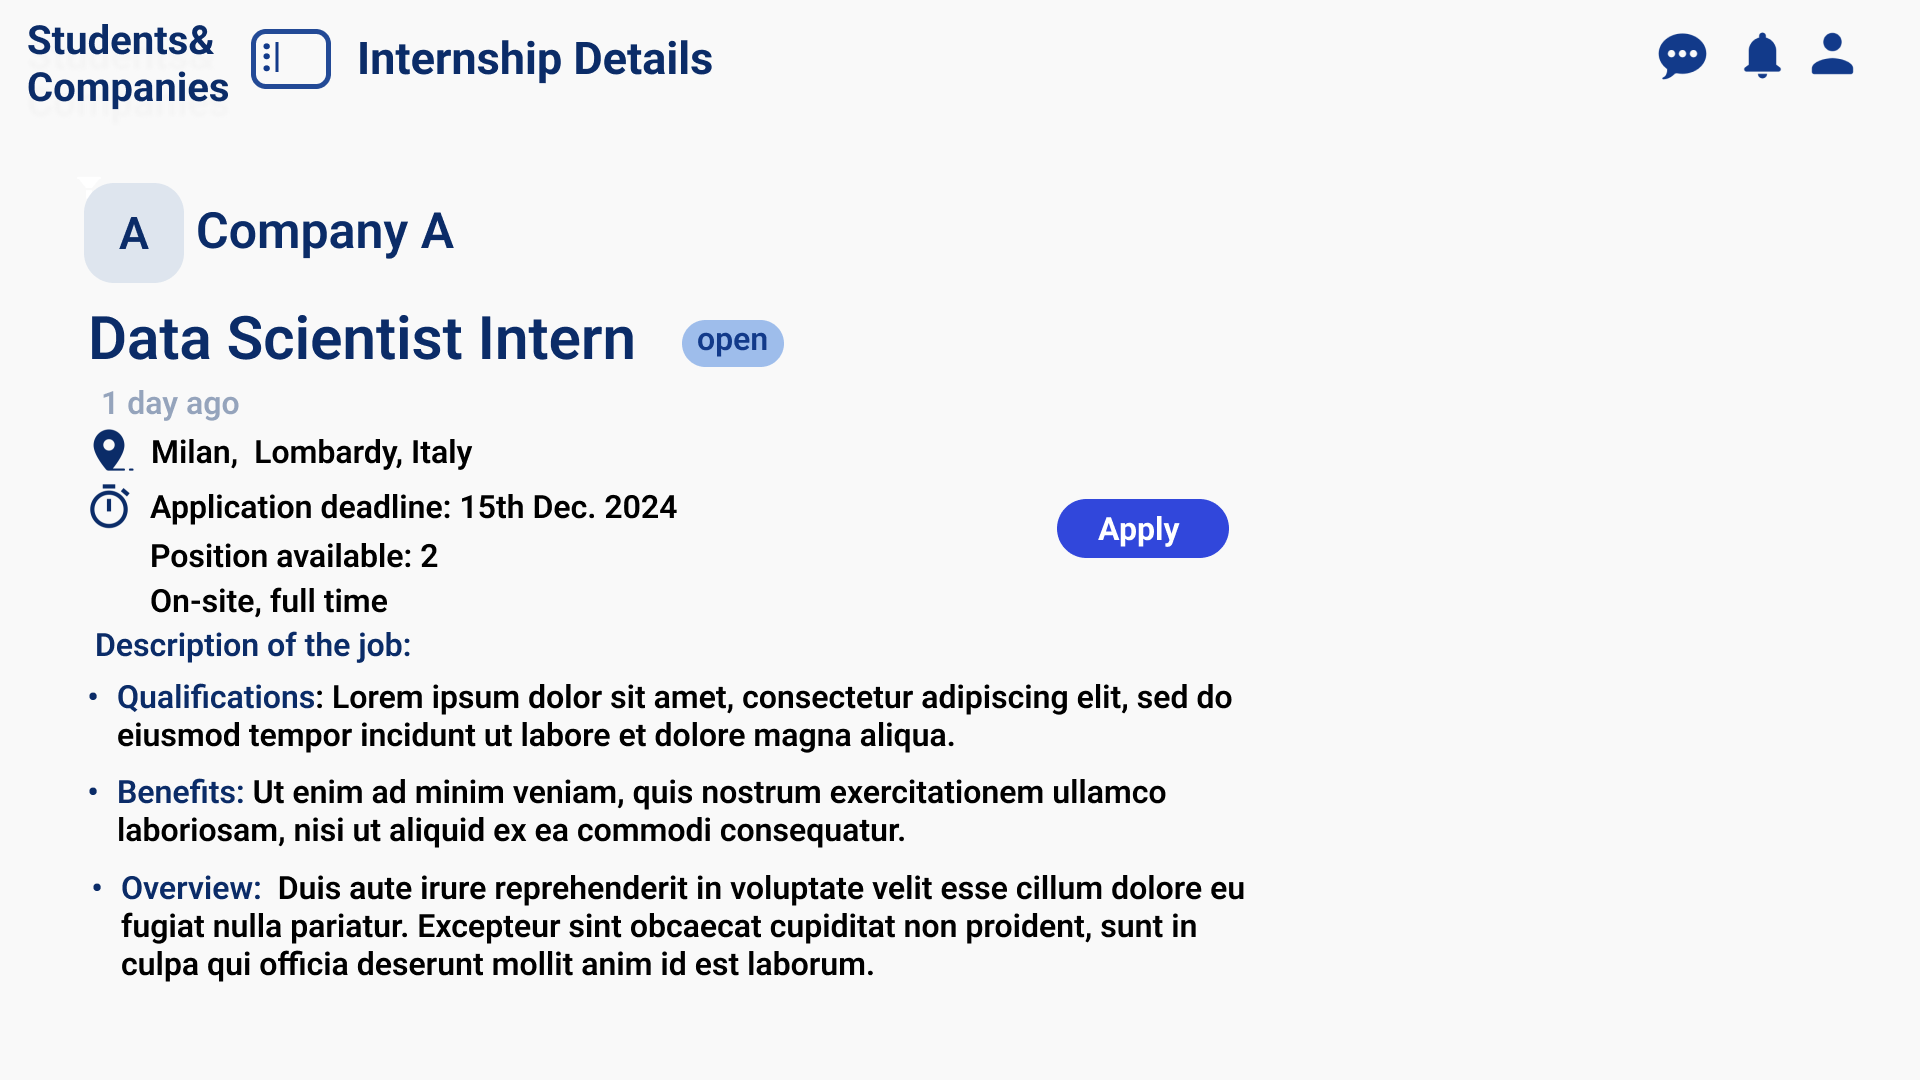
\includegraphics[width=0.8\textwidth]{Images/UI/Internship details-student view.png}
    \caption{Internship announcement details }\label{fig:Internship announcement details}
\end{figure}
\subsubsection{Student profile page}
It shows a student's profile from the prospective of other's user once looking for his/her profile.
The personal information such as profile photo, name, email and major are displayed in this page as 
well as the list of internships the student has participated. 
\begin{figure}[H]
    \centering
    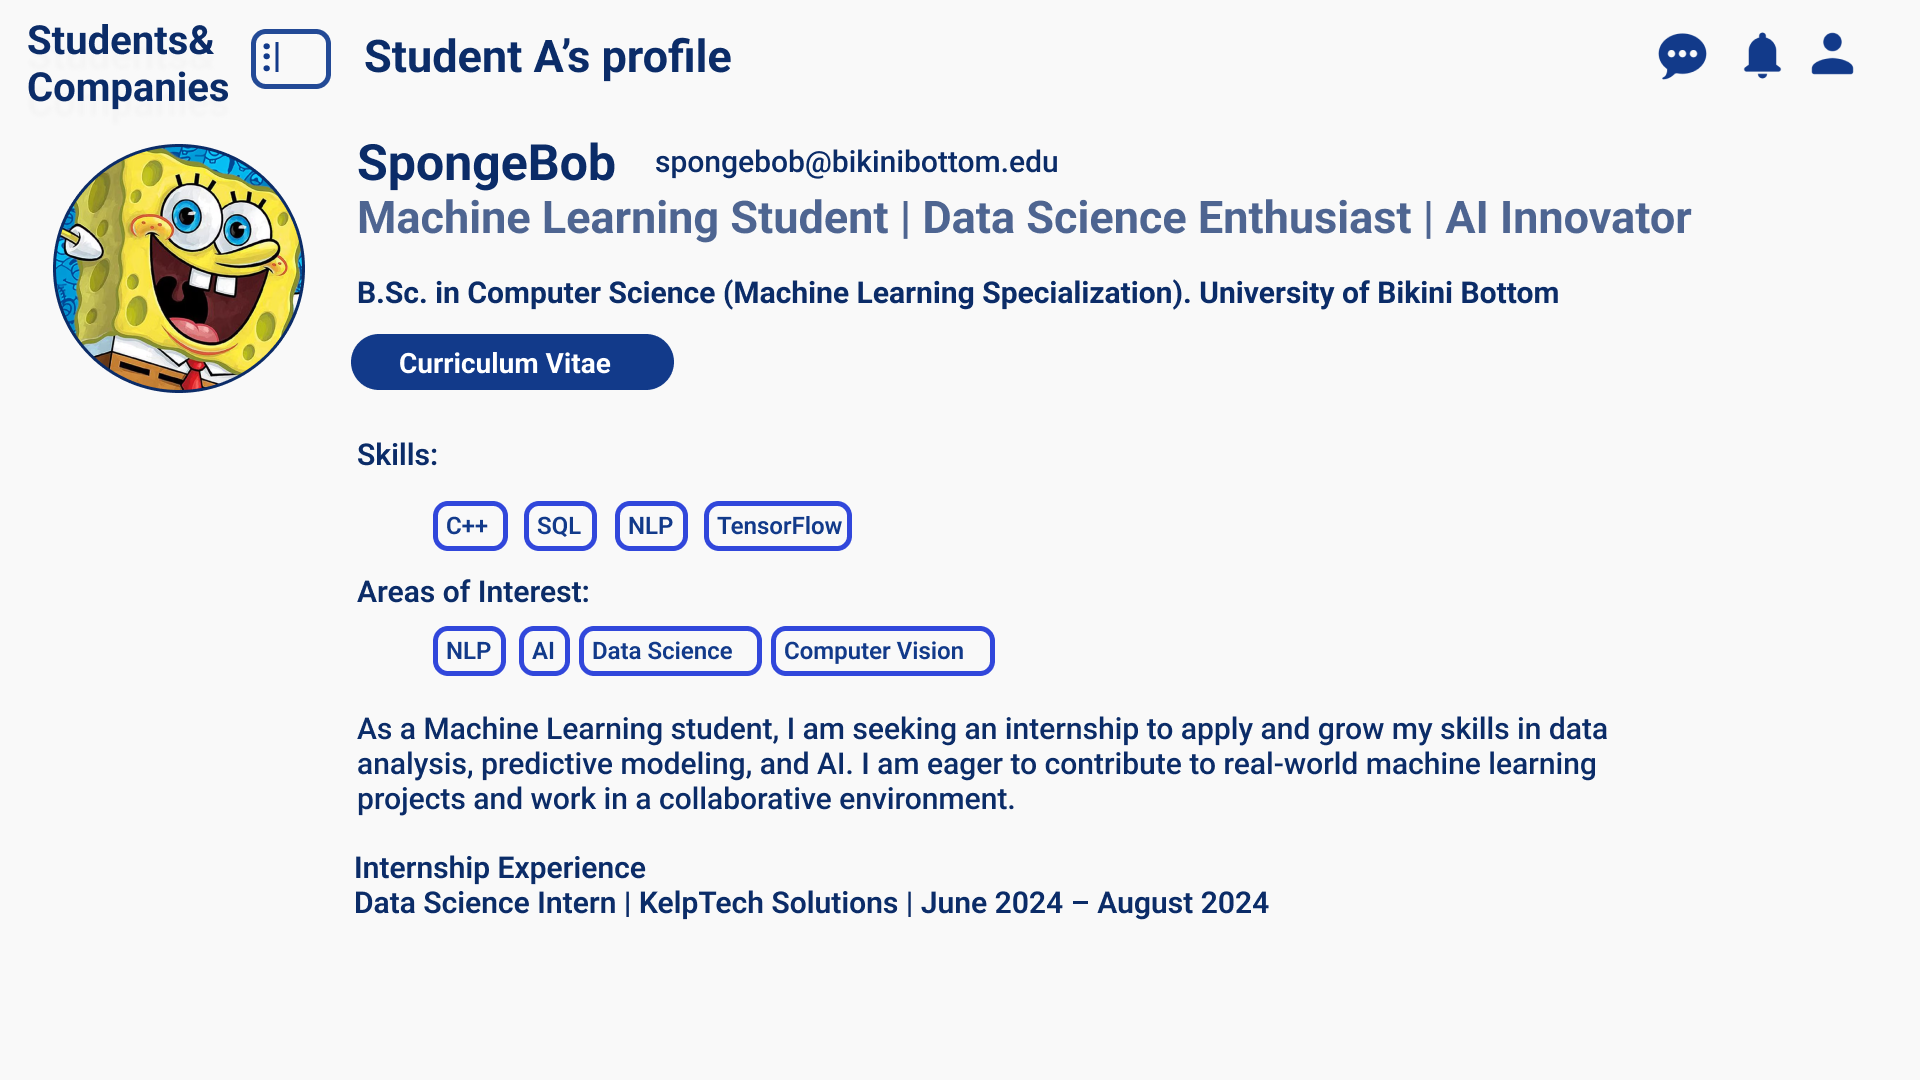
\includegraphics[width=0.8\textwidth]{Images/UI/Student profile.png}
    \caption{Student's profile from other's view}\label{fig:Student's profile from other's view}
\end{figure}

\newpage
\subsection{Company's view}
As the student, the company can use the side menu to navigate to the desired page:
\textit{Search},\textit{Dashboard},\textit{Publish Internship},\textit{Internship Management}.
\begin{figure}[H]
    \centering
    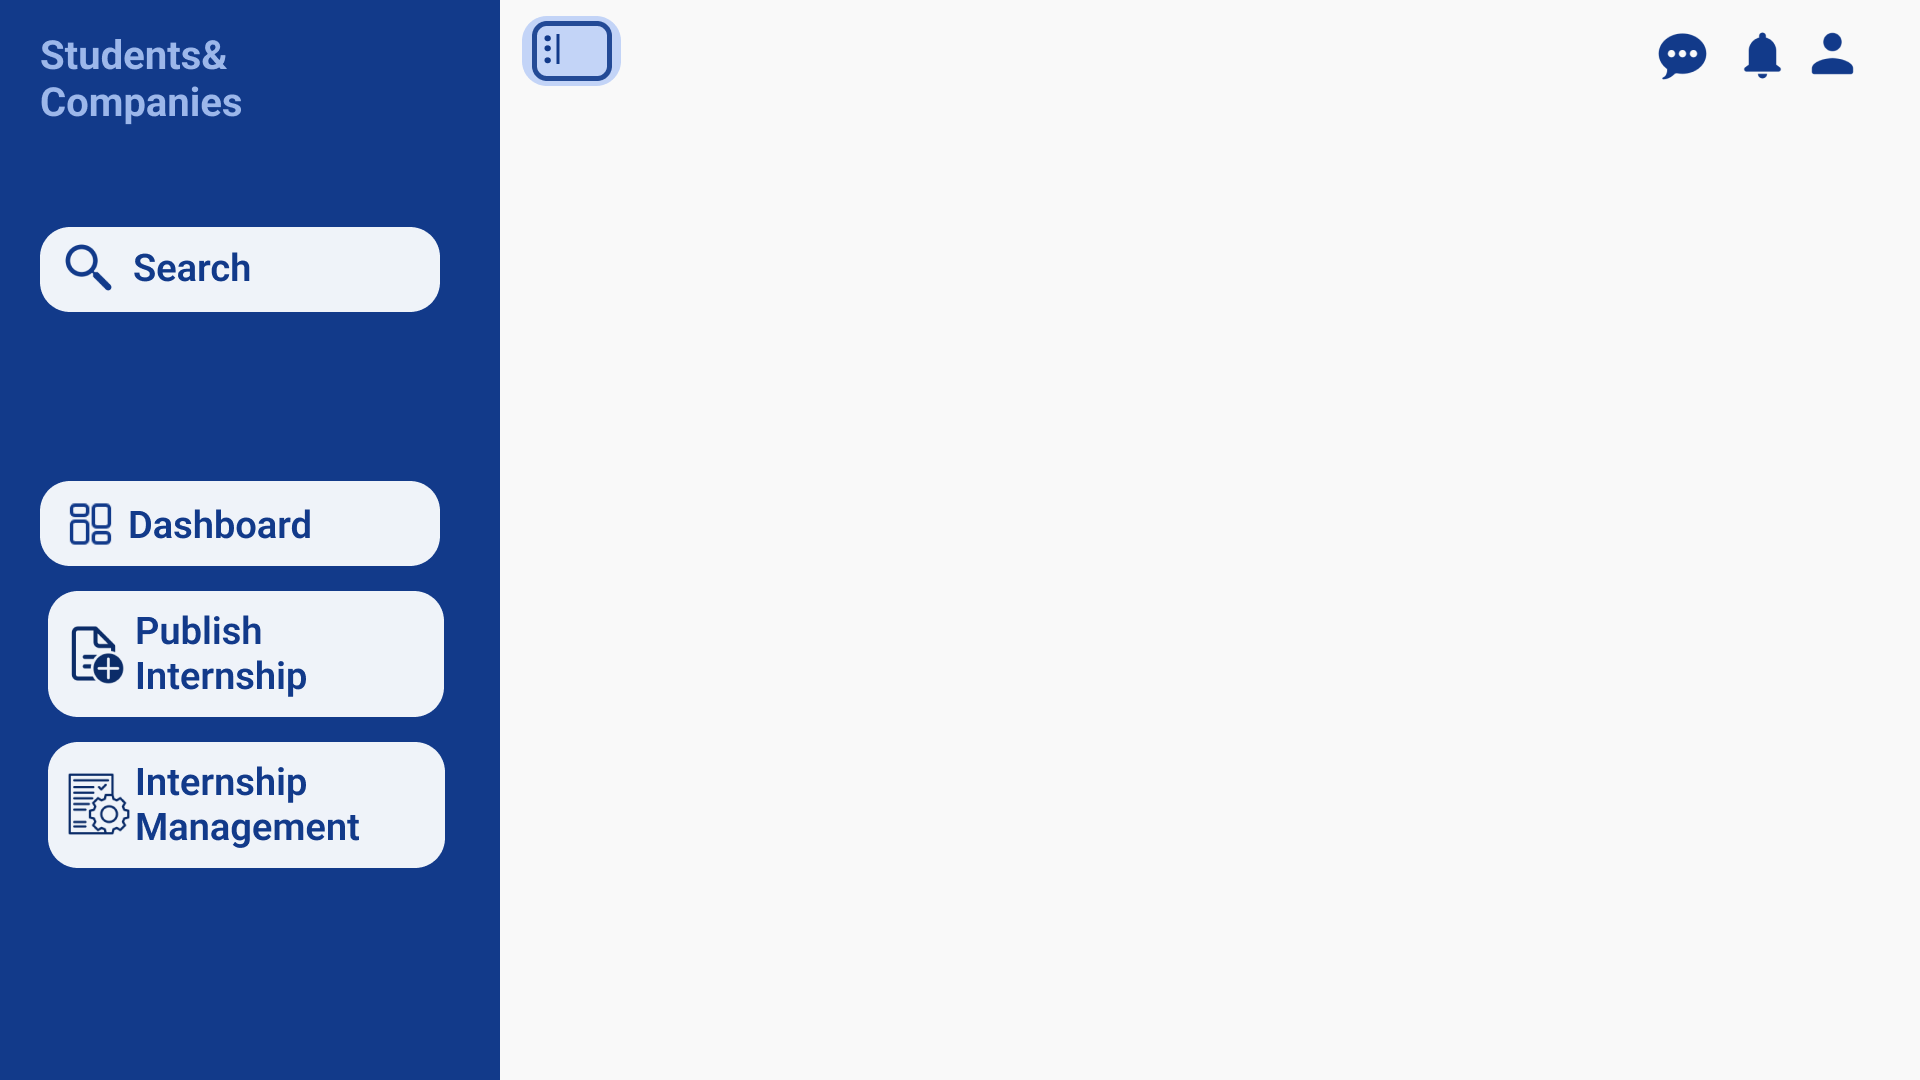
\includegraphics[width=0.8\textwidth]{Images/UI/Layout-Company.png}
    \caption{Company's Side Menu}\label{fig:Company_view}
\end{figure}
\subsubsection{Dashboard page}
Similar to the student's view, the company is directed to the Dashboard page upon logging in.
At the top of the page, the company can use the search bar as well as the search bar presented in the student's view.\\
The Dashboard provides an overview that allows companies to quickly assess the announcements they have published
and allows them to access directly to the publish internship page by clicking on the \textit{Publish new internship} button.\\
Below that, there is a section In progress internship overview that allows companies to monitor the status of the internships in progress 
and clicking on the open button will redirect the company to the feedback and complaint page for the that internship.\\
\begin{figure}[H]
    \centering
    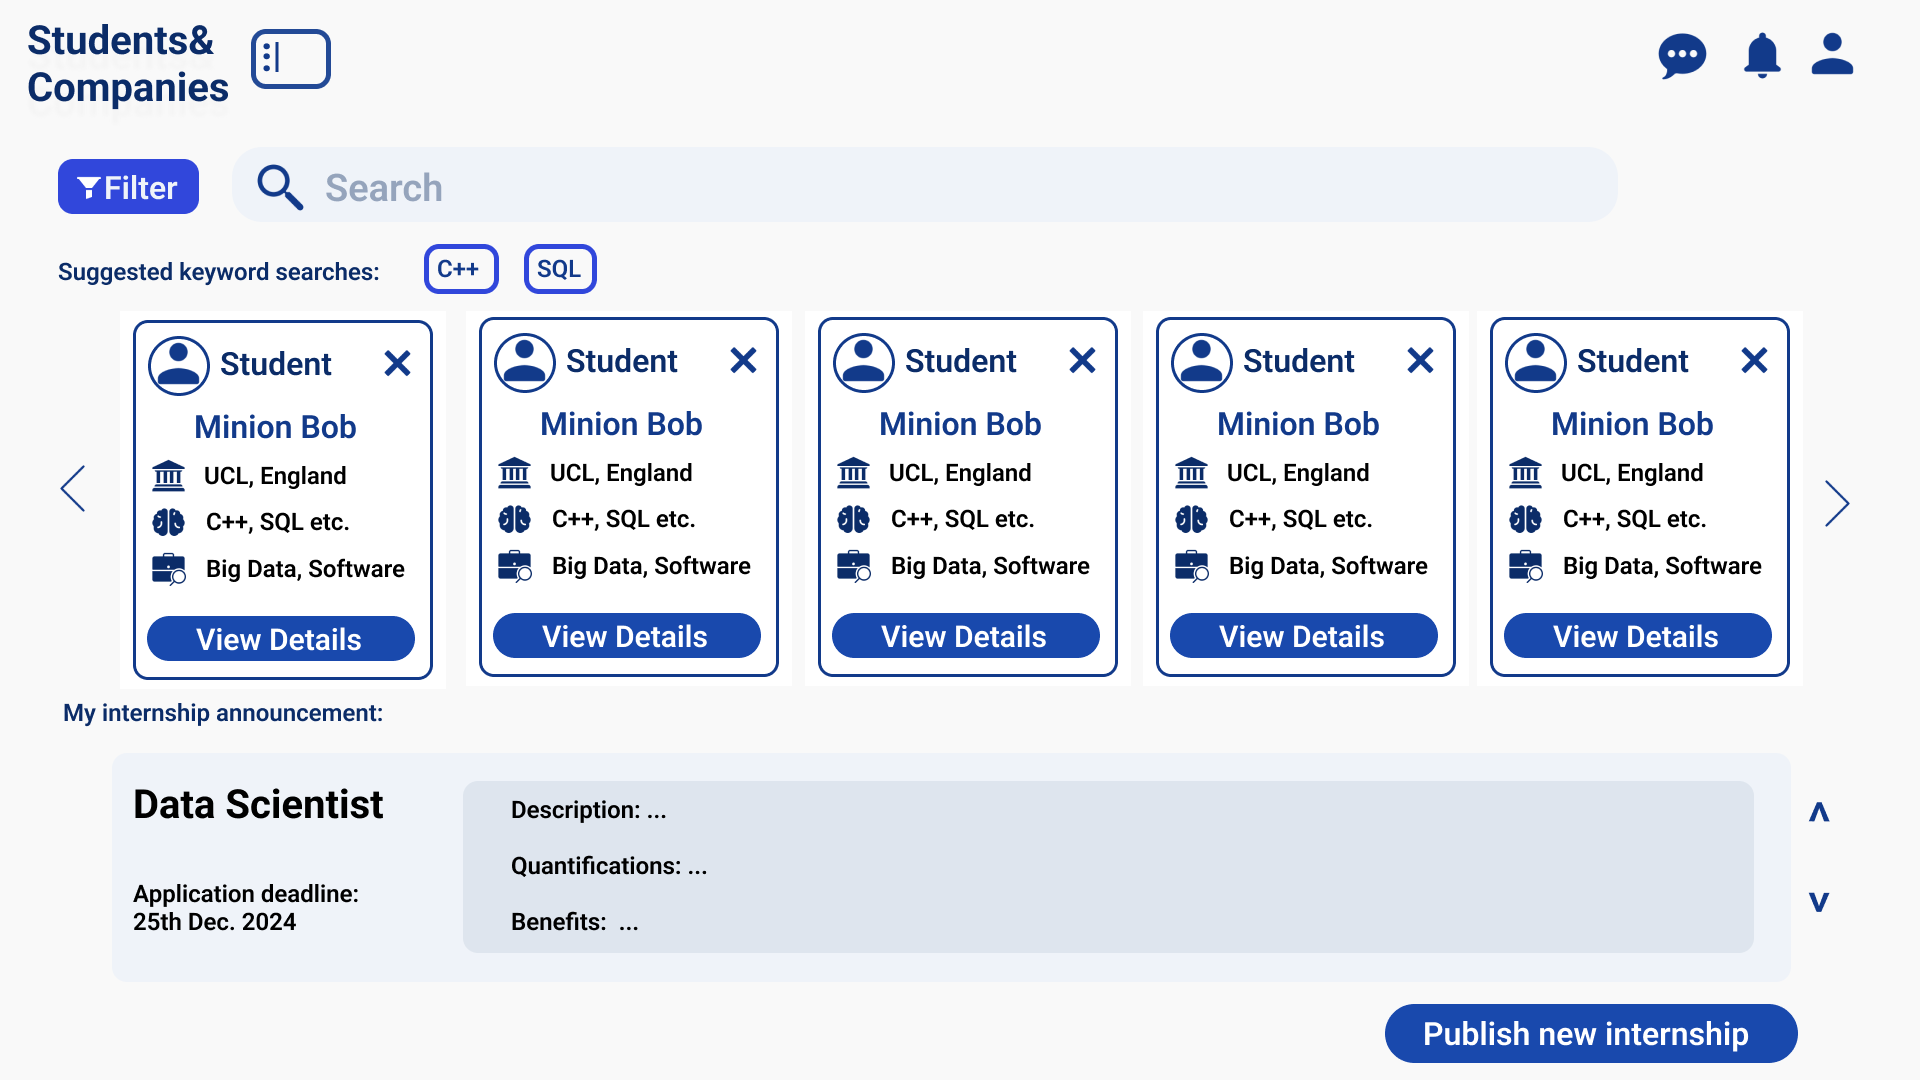
\includegraphics[width=0.8\textwidth]{Images/UI/Dashboard 1-company.png}
    \caption{Company's Dashboard 1}\label{fig:DashboardCompany1}
\end{figure}

\begin{figure}[H]
    \centering
    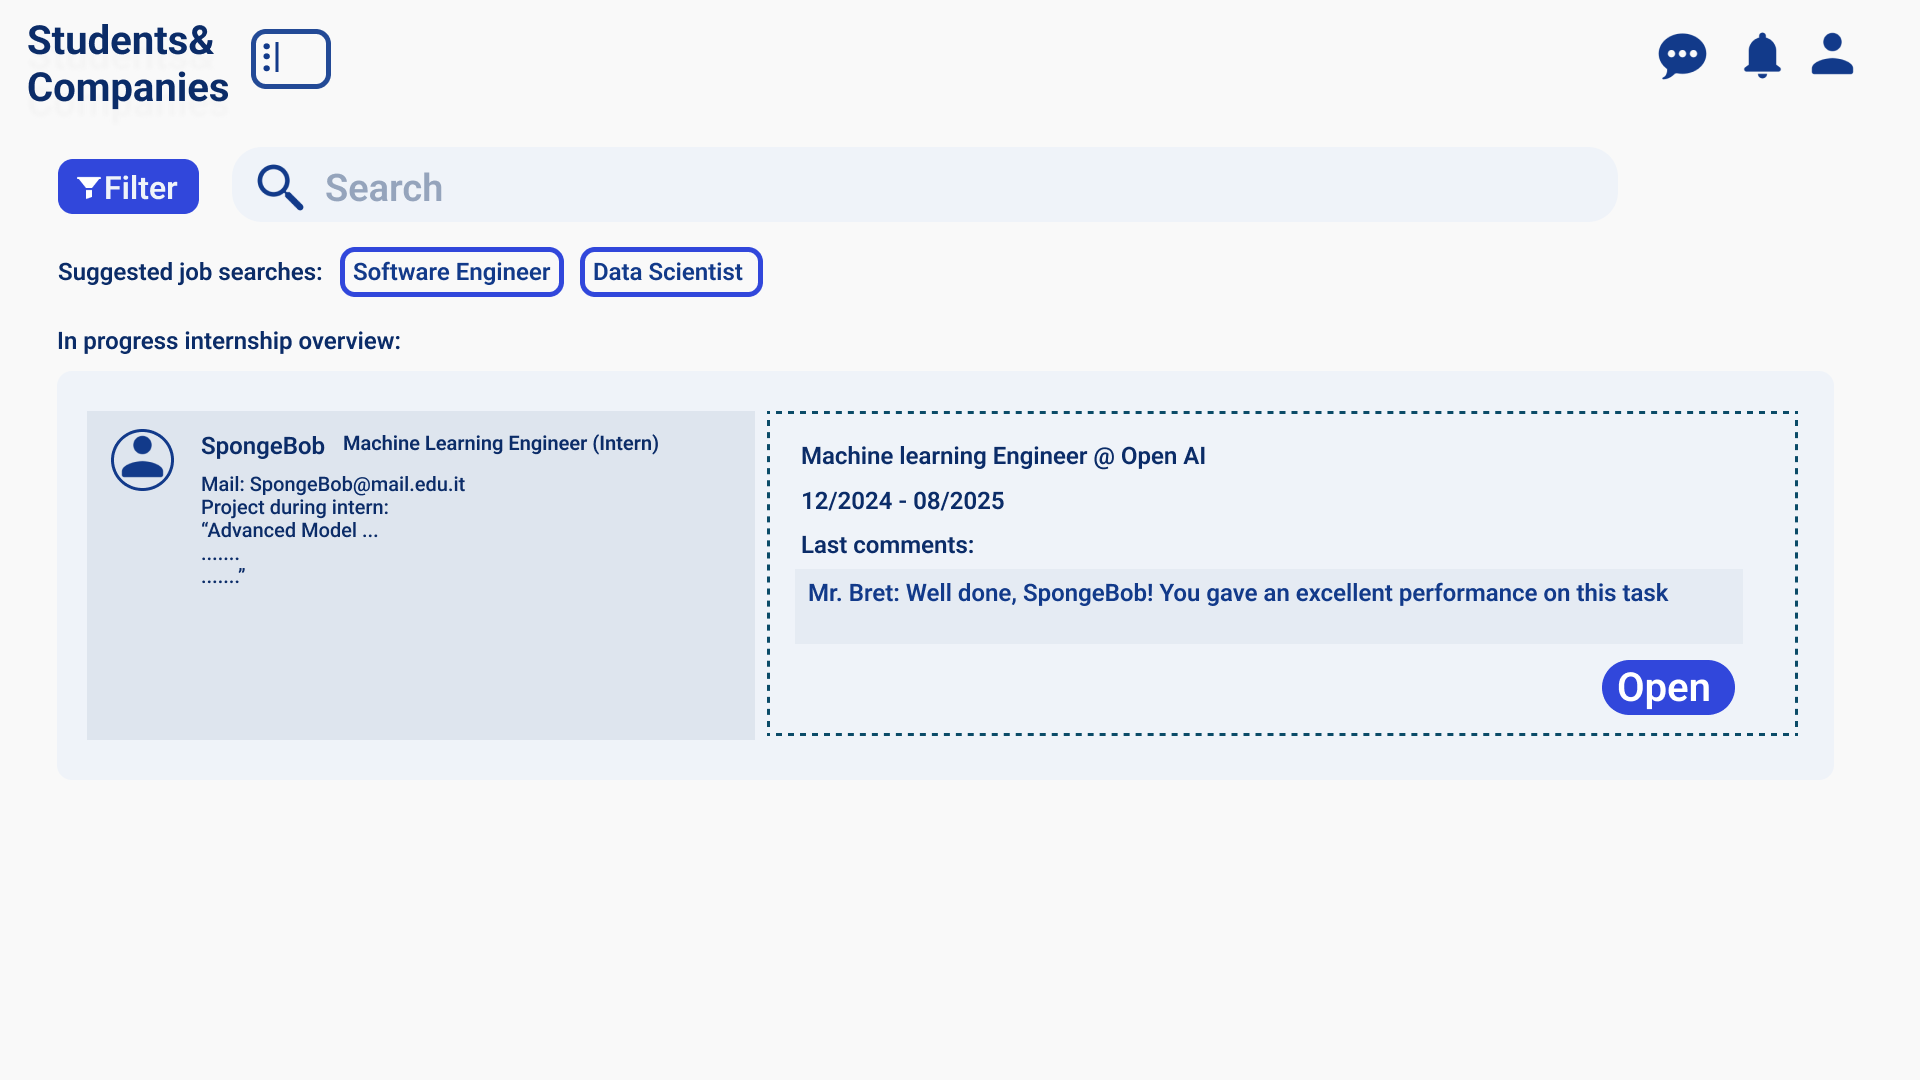
\includegraphics[width=0.8\textwidth]{Images/UI/Dashboard 2-company.png}
    \caption{Company's Dashboard 2}\label{fig:DashboardCompany2}
\end{figure}
\subsubsection{Publish Internship page}
In this page, the company can fill in the required information to publish a new internship announcement on the platform.
\begin{figure}[H]
    \centering
    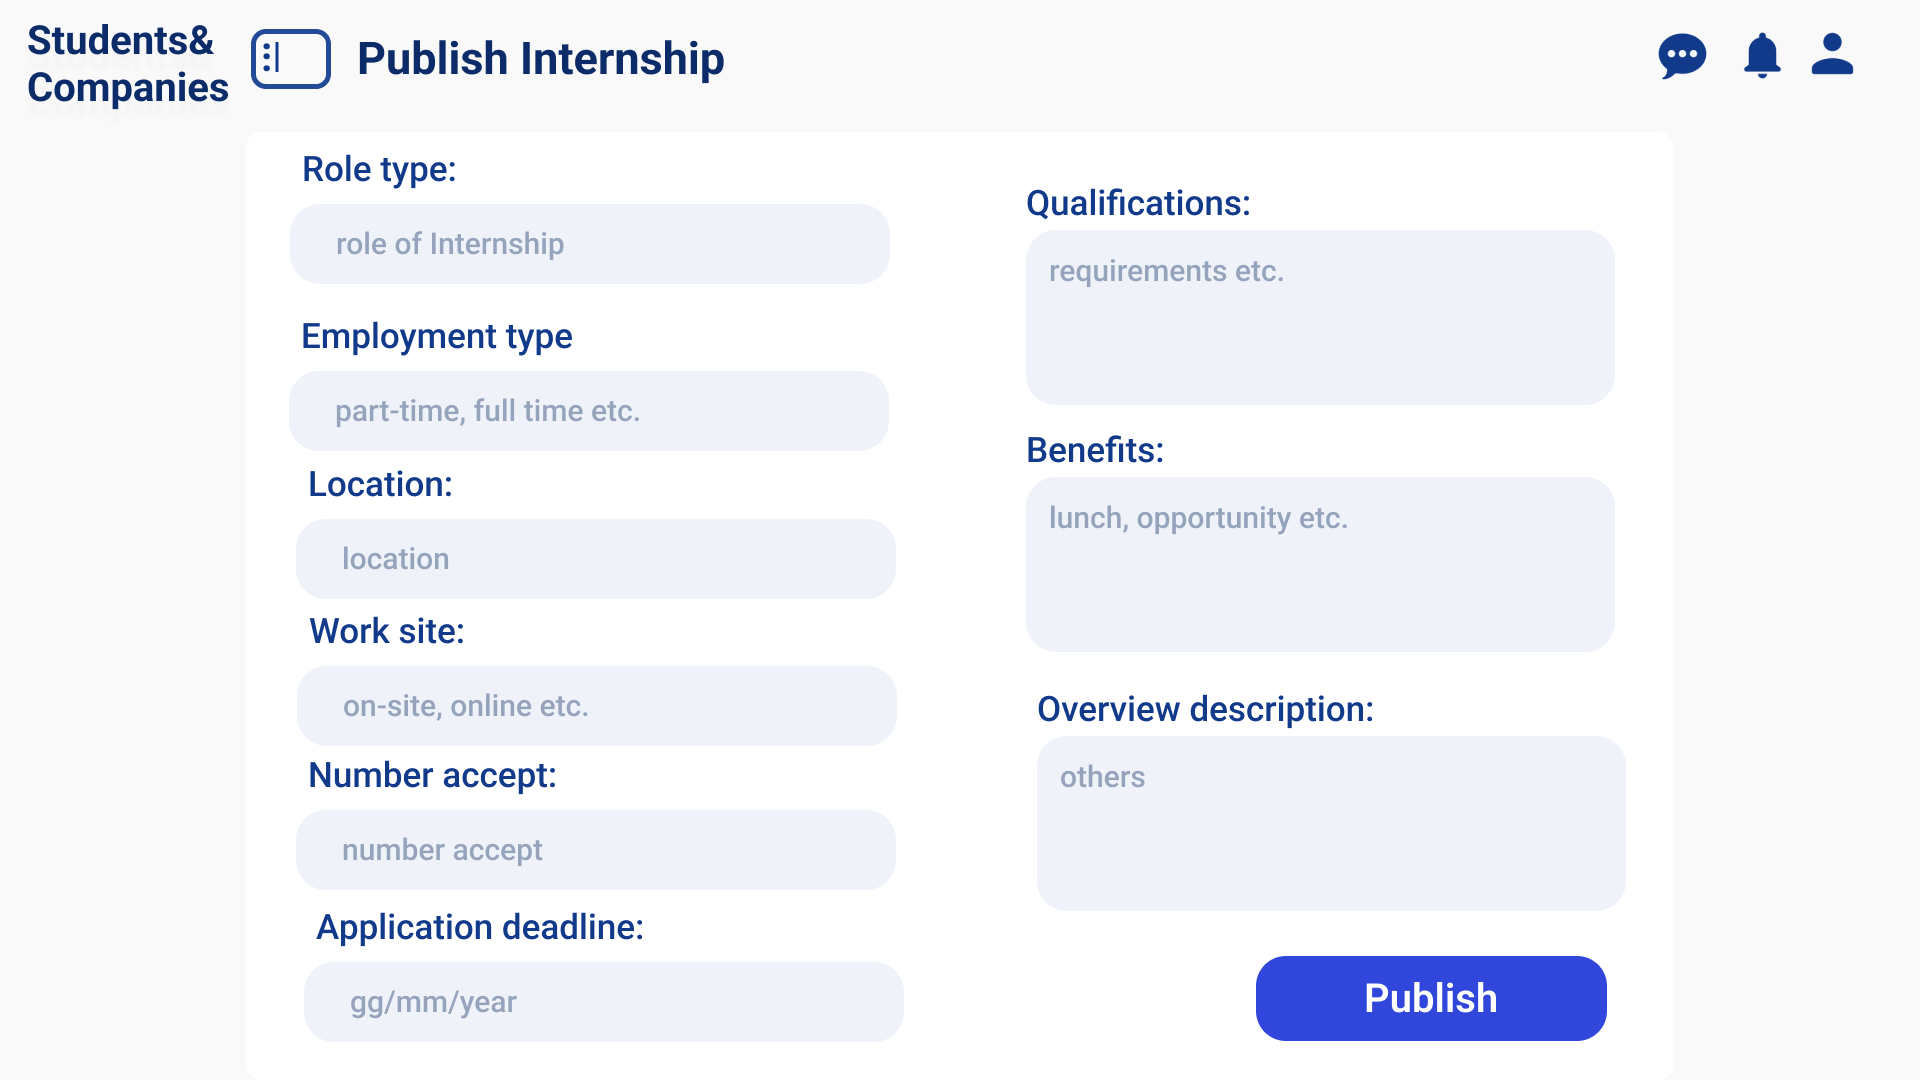
\includegraphics[width=0.8\textwidth]{Images/UI/Publish Internship -company.png}
    \caption{Publish Internship}\label{fig:Publish Internship}
\end{figure}

\subsubsection{Internship Management page}
Here in figure\ref{fig:Internship Management 1}, the company can view the list of internships they have published and take action based on the status of the internship:
\begin{itemize}
    \item[-] In publishing, means the internship announcement is still open for students to apply, the company can click on the \textit{View details} button to view the page with details of the internship announcement, figure\ref{fig:Internship details in publishing phase}.
    \item[-] In selection, means the deadline is reached and the internship enter in selection phase, the company can click on the 
    \textit{Select candidates} button to view the list of candidates who have applied for the internship and take action to select 
    the candidates to process the interview, figure\ref{fig:Select candidates}.
    \item[-] In progress, means that internship is in progress, the company can click on the \textit{Add comments} button to access the feedback and complaints page for the internship, figure\ref{fig:Feedback and Complaint}.
    \item[-] Completed, means that internship is finished, the company can click on the \textit{View details} button to view the announcement details and feedback and complaints recorded by the company and the student during the internship.
\end{itemize}

\begin{figure}[H]
    \centering
    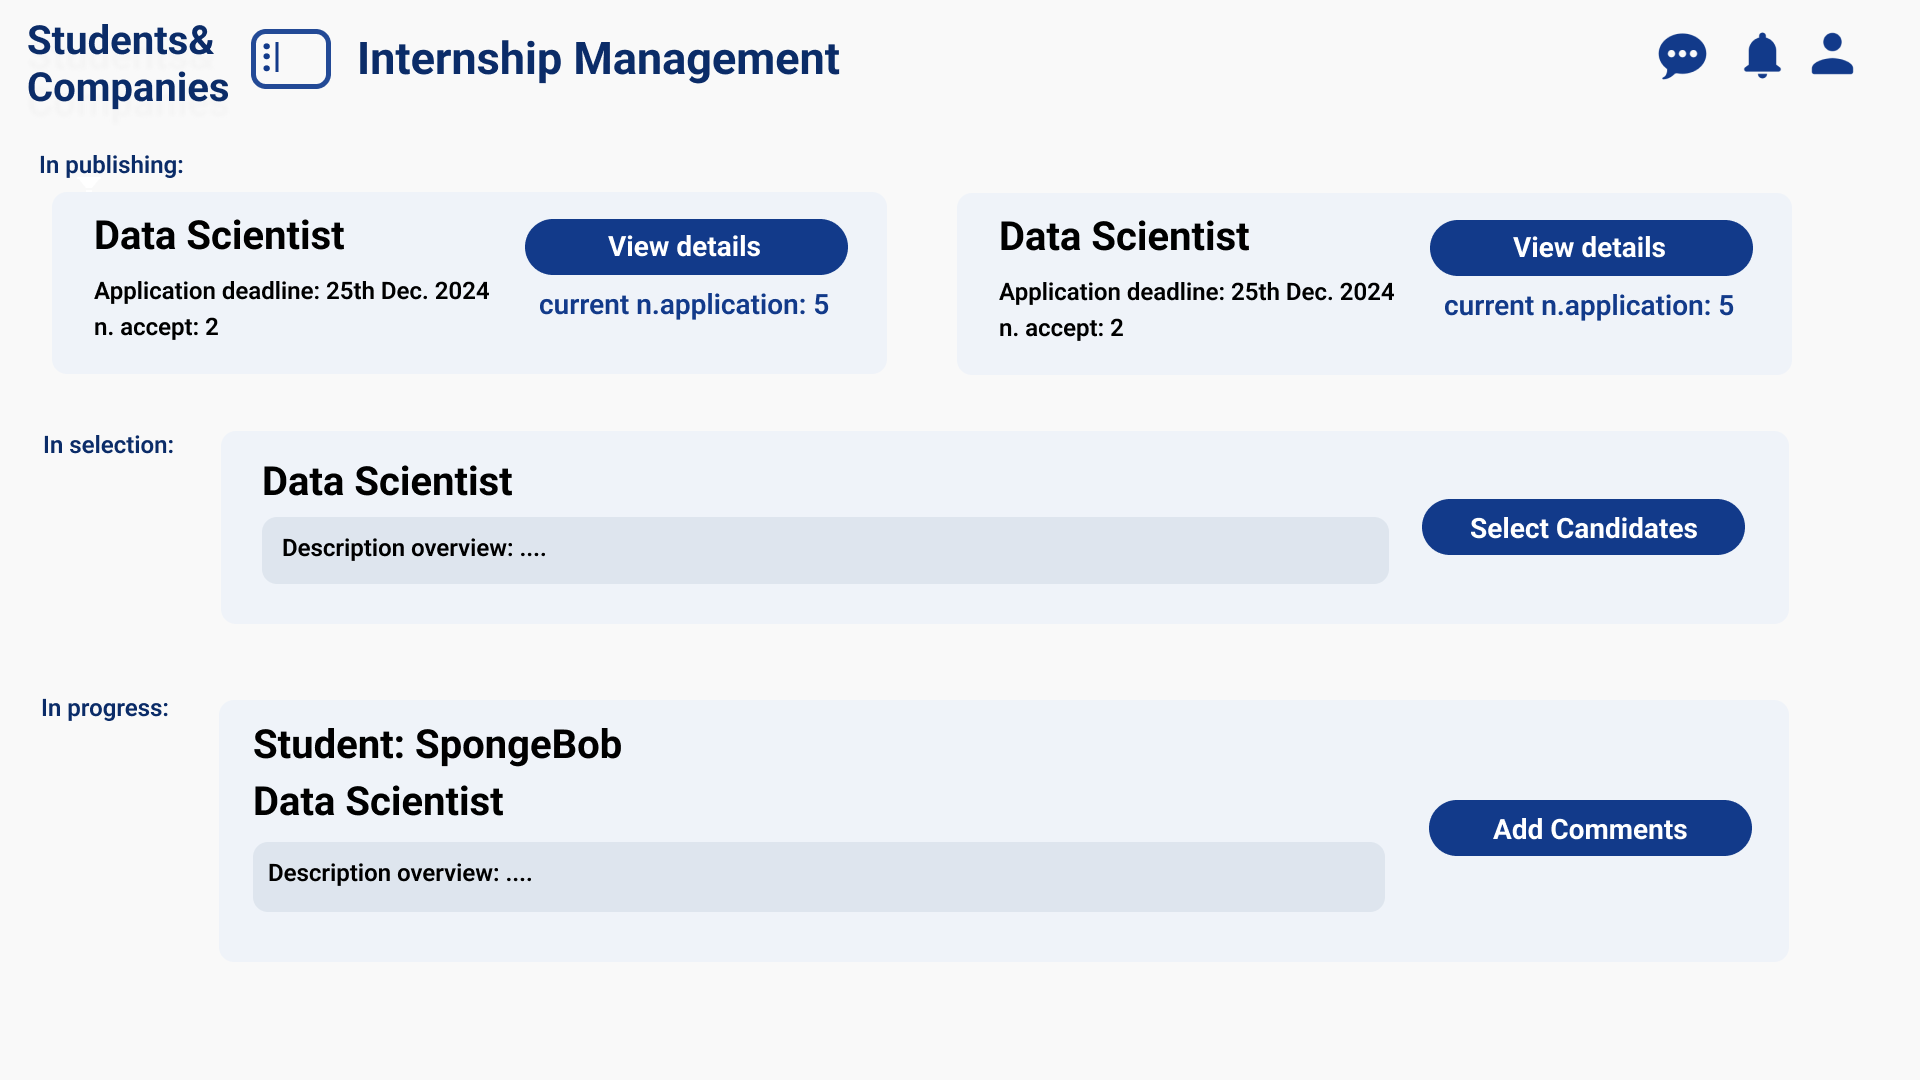
\includegraphics[width=0.8\textwidth]{Images/UI/Internship Management-company.png}
    \caption{Internship Management 1}\label{fig:Internship Management 1}
\end{figure}

\begin{figure}[H]
    \centering
    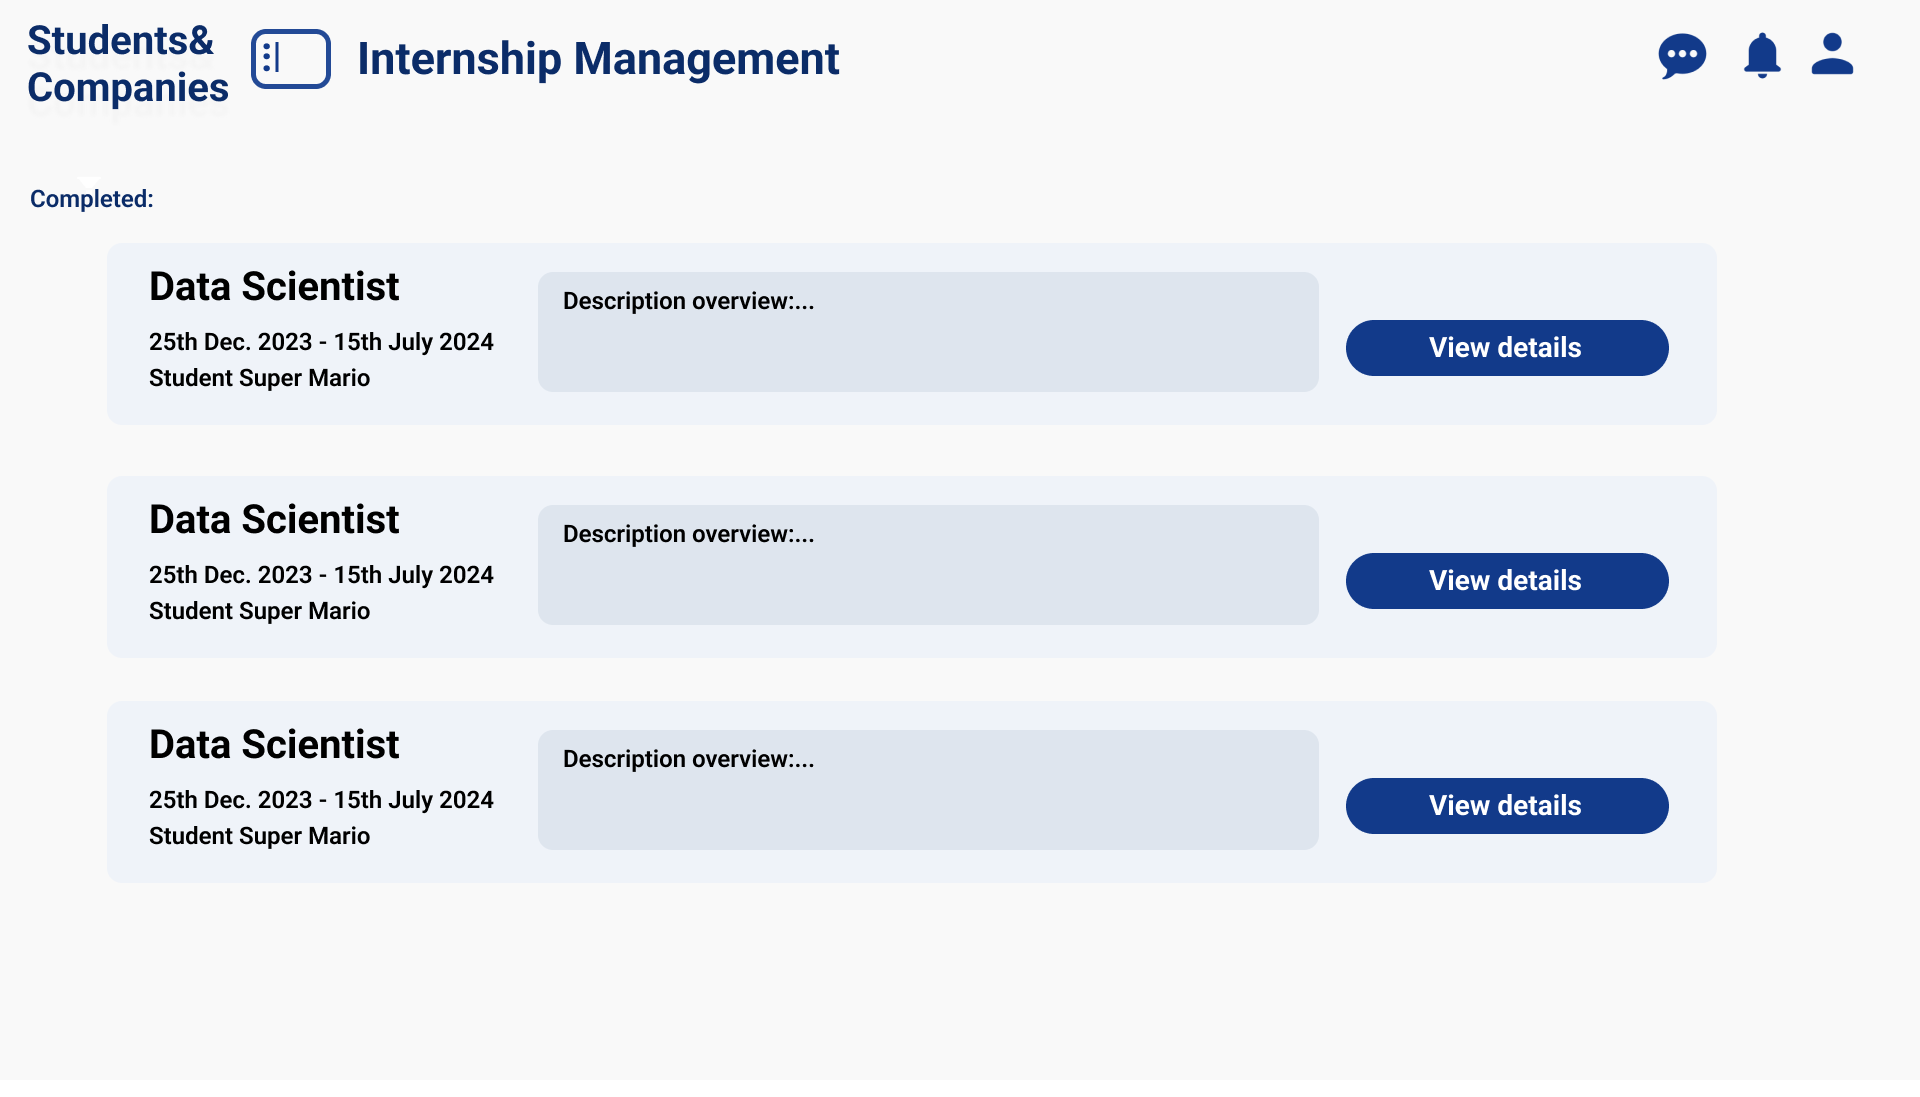
\includegraphics[width=0.8\textwidth]{Images/UI/Internship Management2-company.png}
    \caption{Internship Management 2}\label{fig:Internship Management 2}
\end{figure}

\subsubsection{Internship details page}
The internship details page in selection phase, the company can view the list of candidates who 
have applied for the internship and select the candidates to process the interview by clicking on the button \textit{process interview}.
\begin{figure}[H]
    \centering
    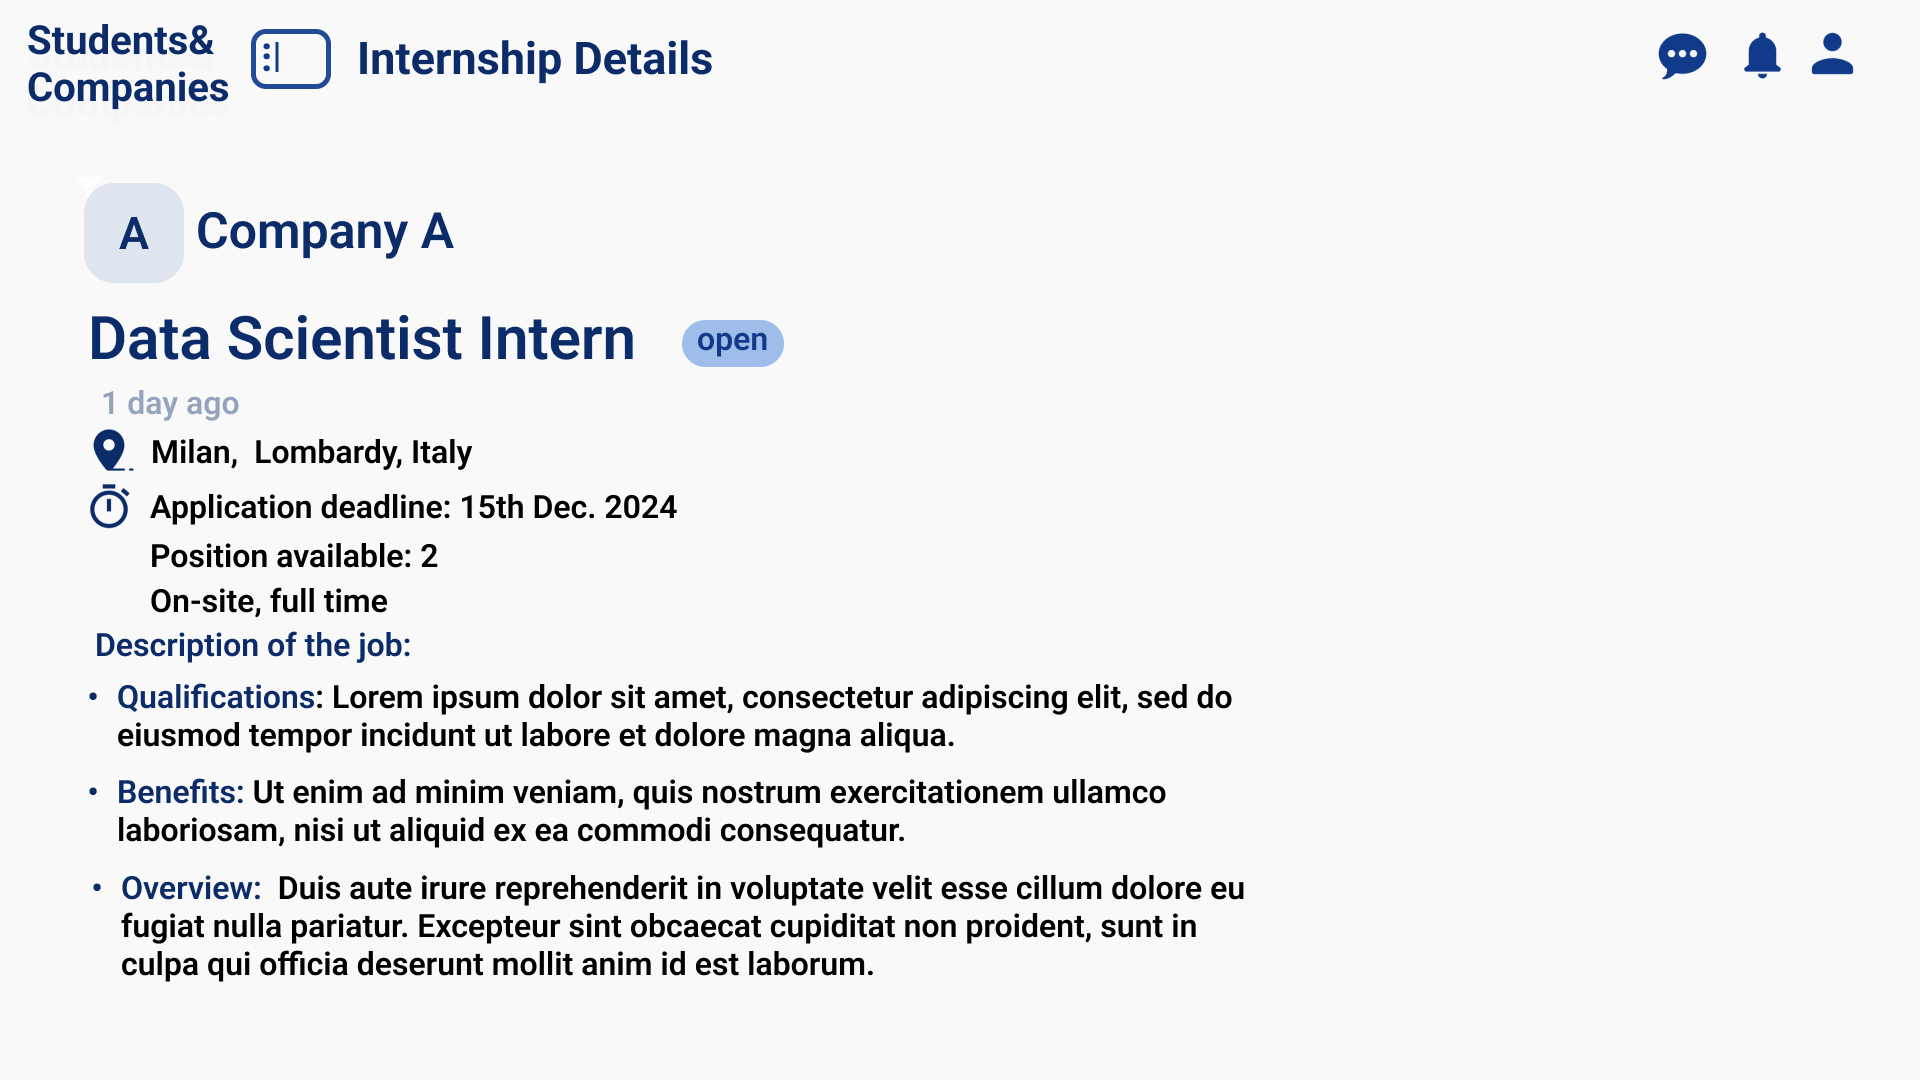
\includegraphics[width=0.8\textwidth]{Images/UI/Internship details-company view.png}
    \caption{Internship details in publishing phase}\label{fig:Internship details in publishing phase}
\end{figure}
\begin{figure}[H]
    \centering
    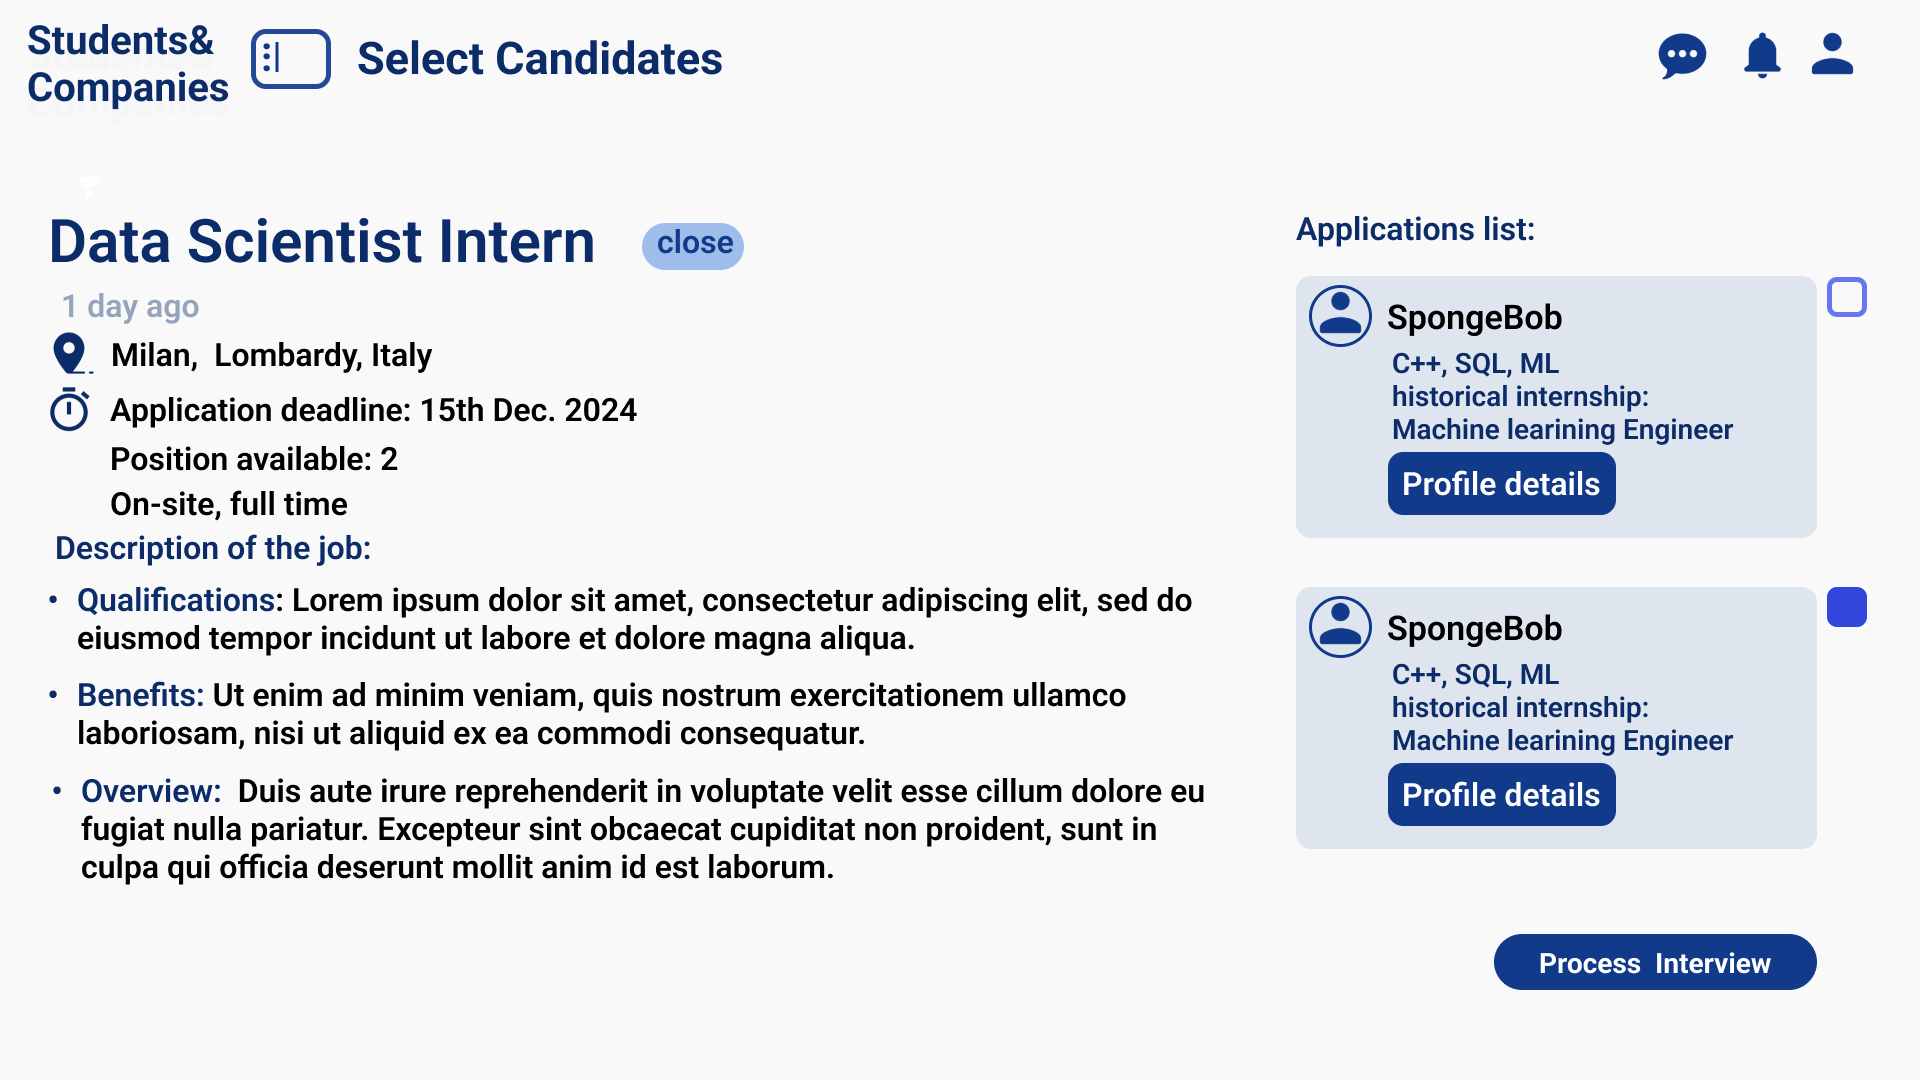
\includegraphics[width=0.8\textwidth]{Images/UI/Select candidates.png}
    \caption{Select candidates}\label{fig:Select candidates}
\end{figure}

\subsubsection{Interview set up page}
In this page, the company can write the invitation letter with the necessary information for the interview and prepare
the questionnaire to ask the candidate to fill in before the interview. Clicking on the \textit{Submit} button will send 
the invitation letter and the questionnaire to the student selected for the interview.
\begin{figure}[H]
    \centering
    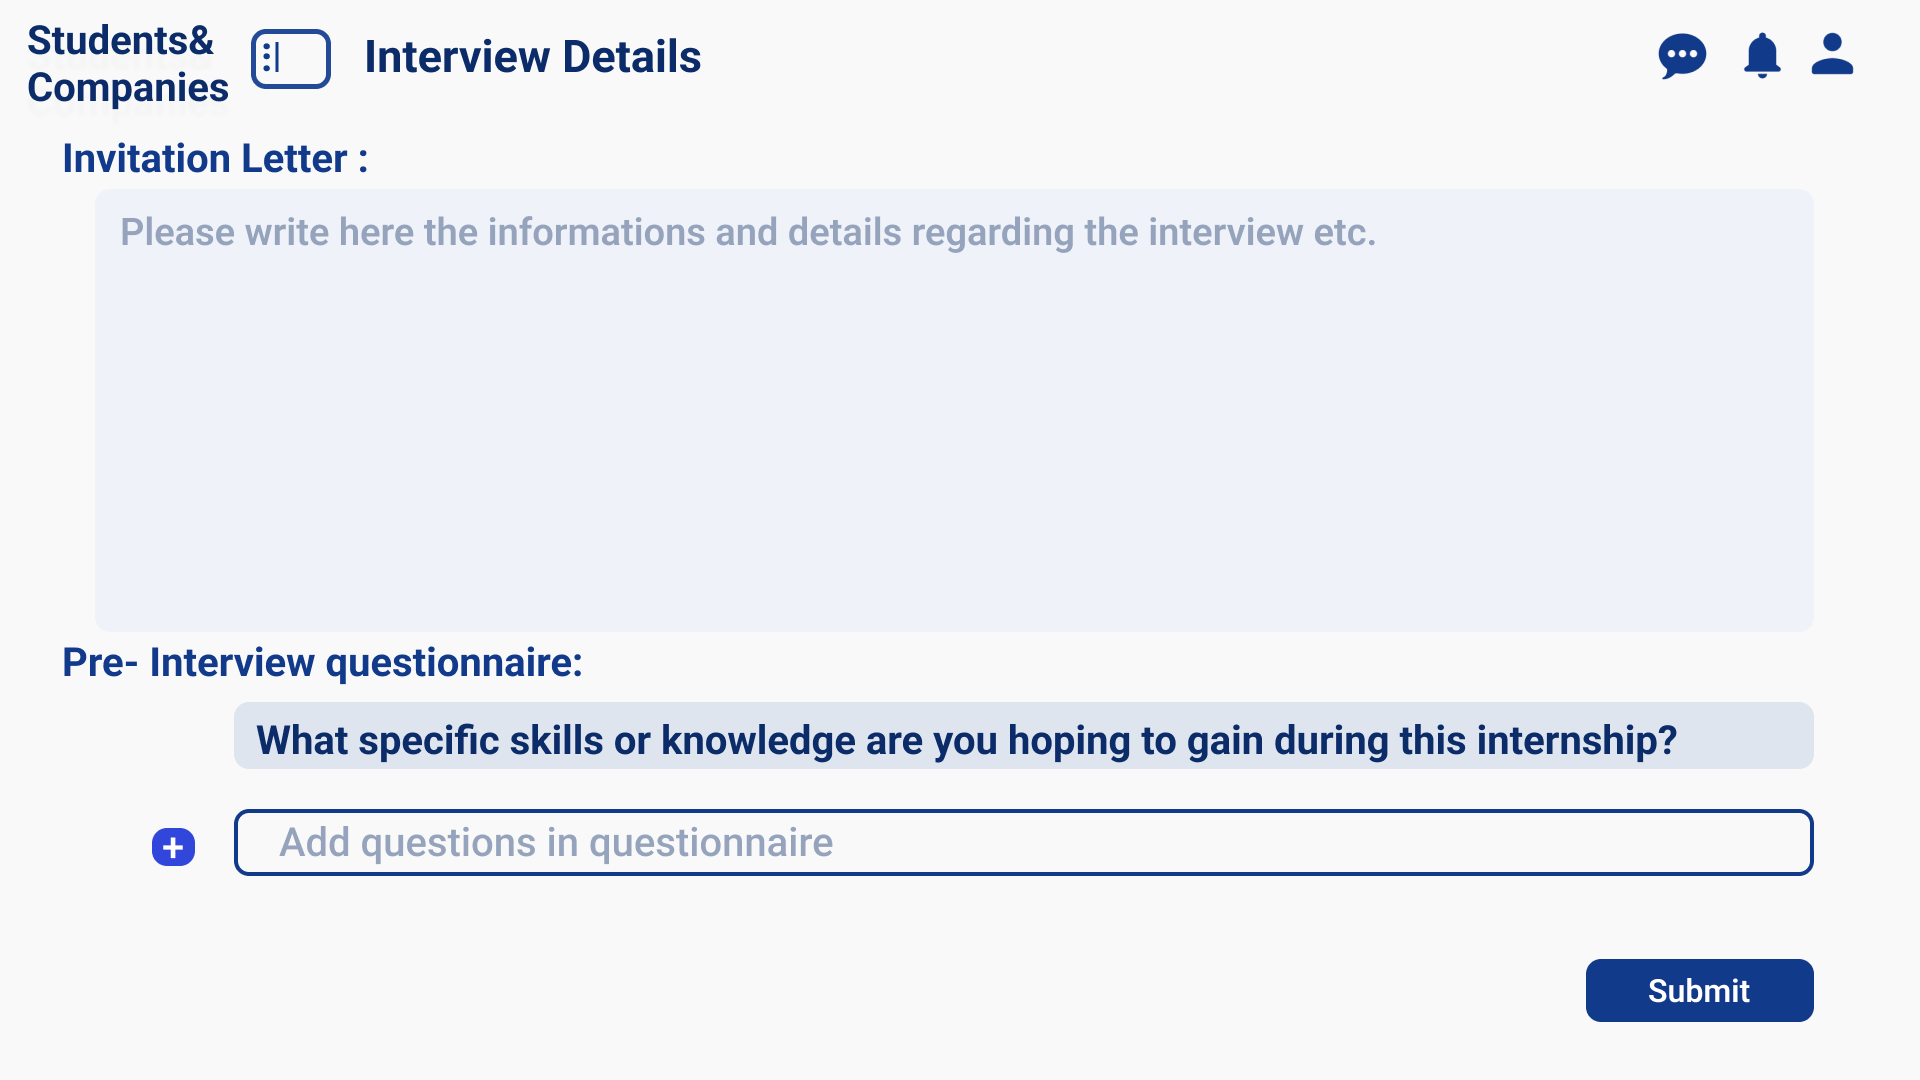
\includegraphics[width=0.8\textwidth]{Images/UI/Set Interview-Company.png}
    \caption{Set up interview}\label{fig:Set up interview}
\end{figure}

\subsubsection{Company profile page}
Figure\ref{fig:Company's profile from other's view} shows a company's profile from the 
prospective of other's user once looking for its profile.
Including the company brief description, contact email, specific fields of the company that 
the company is focusing on and the list of internships the company has published.
\begin{figure}[H]
    \centering
    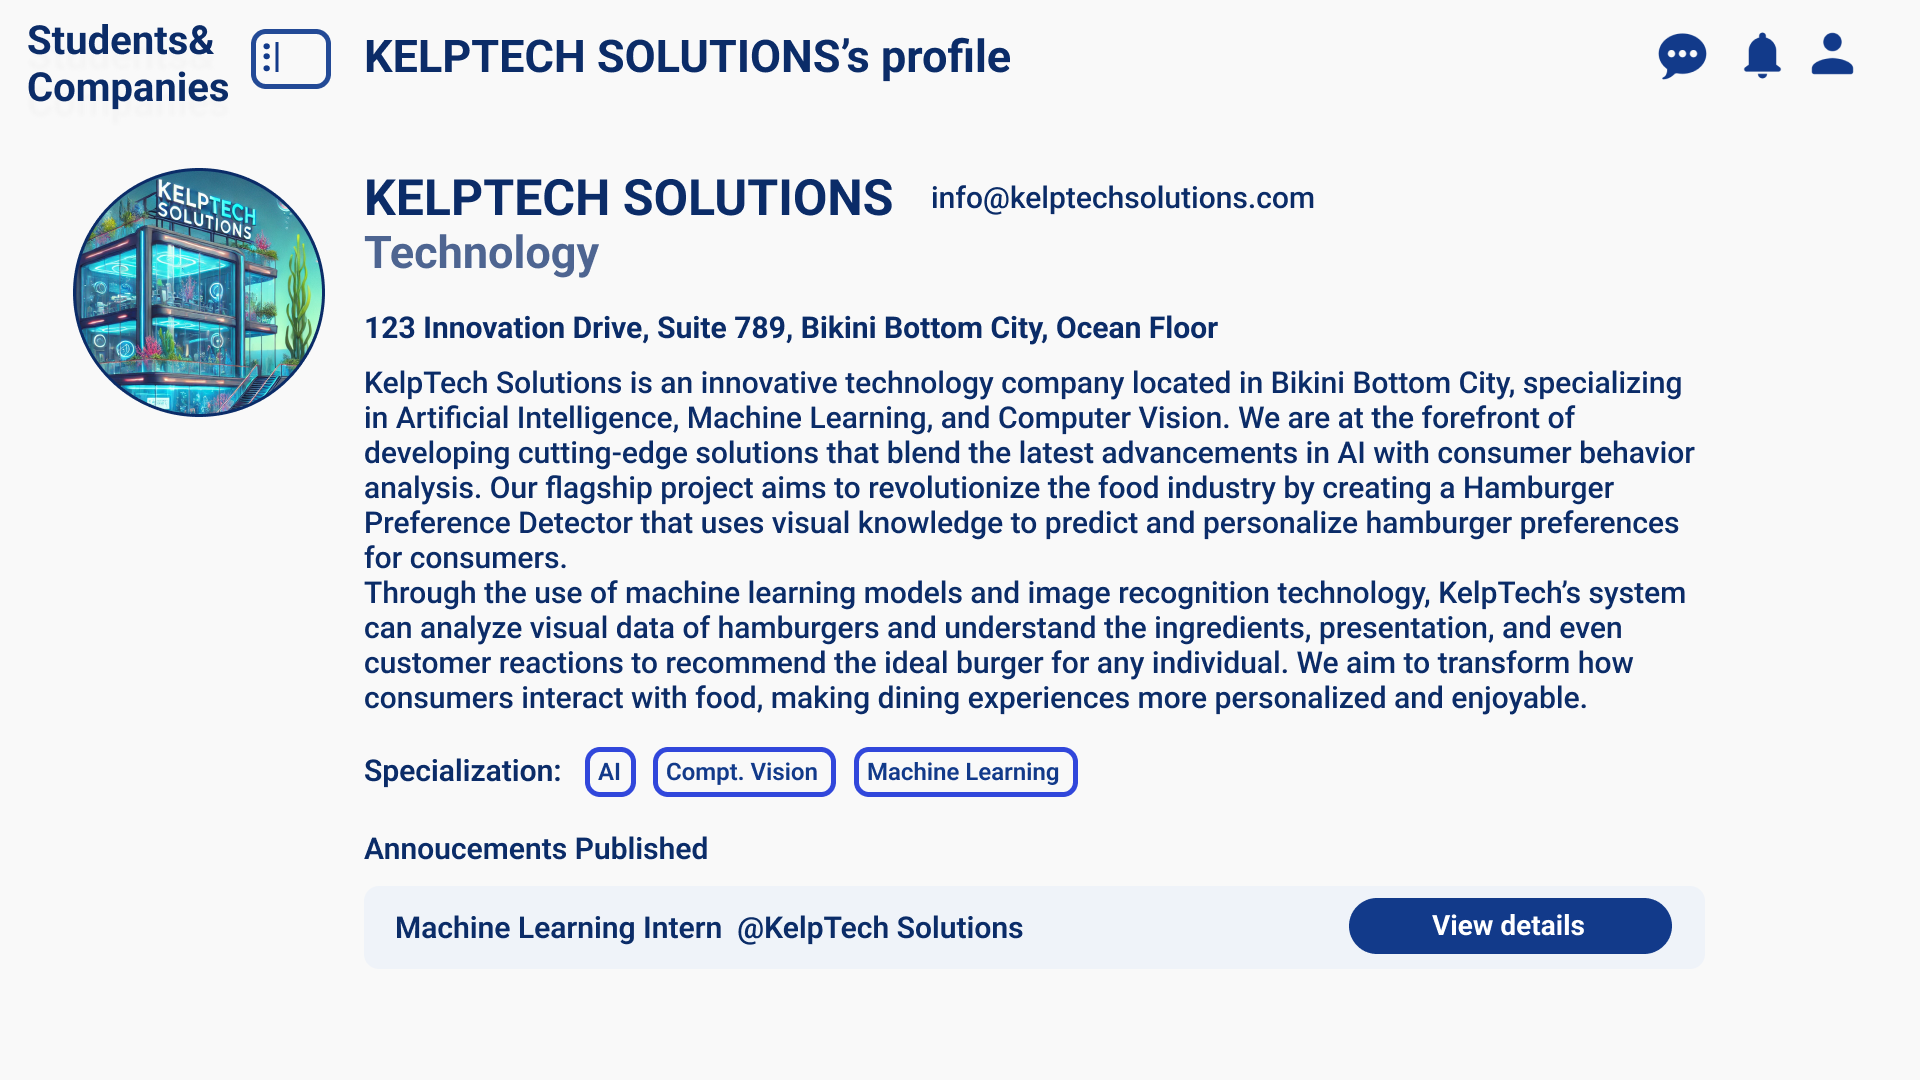
\includegraphics[width=0.8\textwidth]{Images/UI/Company profile.png}
    \caption{Company's profile from other's view}\label{fig:Company's profile from other's view}
\end{figure}

\newpage
\subsection{Student and Company's view}
\subsubsection{FeedBack and Compalint page}
Figure\ref{fig:Feedback and Complaint} shows the page where the involved parties can leave feedback and complaints about the internship.
There are two blocks, one shows the feedback and complaints history and one is the box where the user can 
write the feedback or complaint.
\begin{figure}[H]
    \centering
    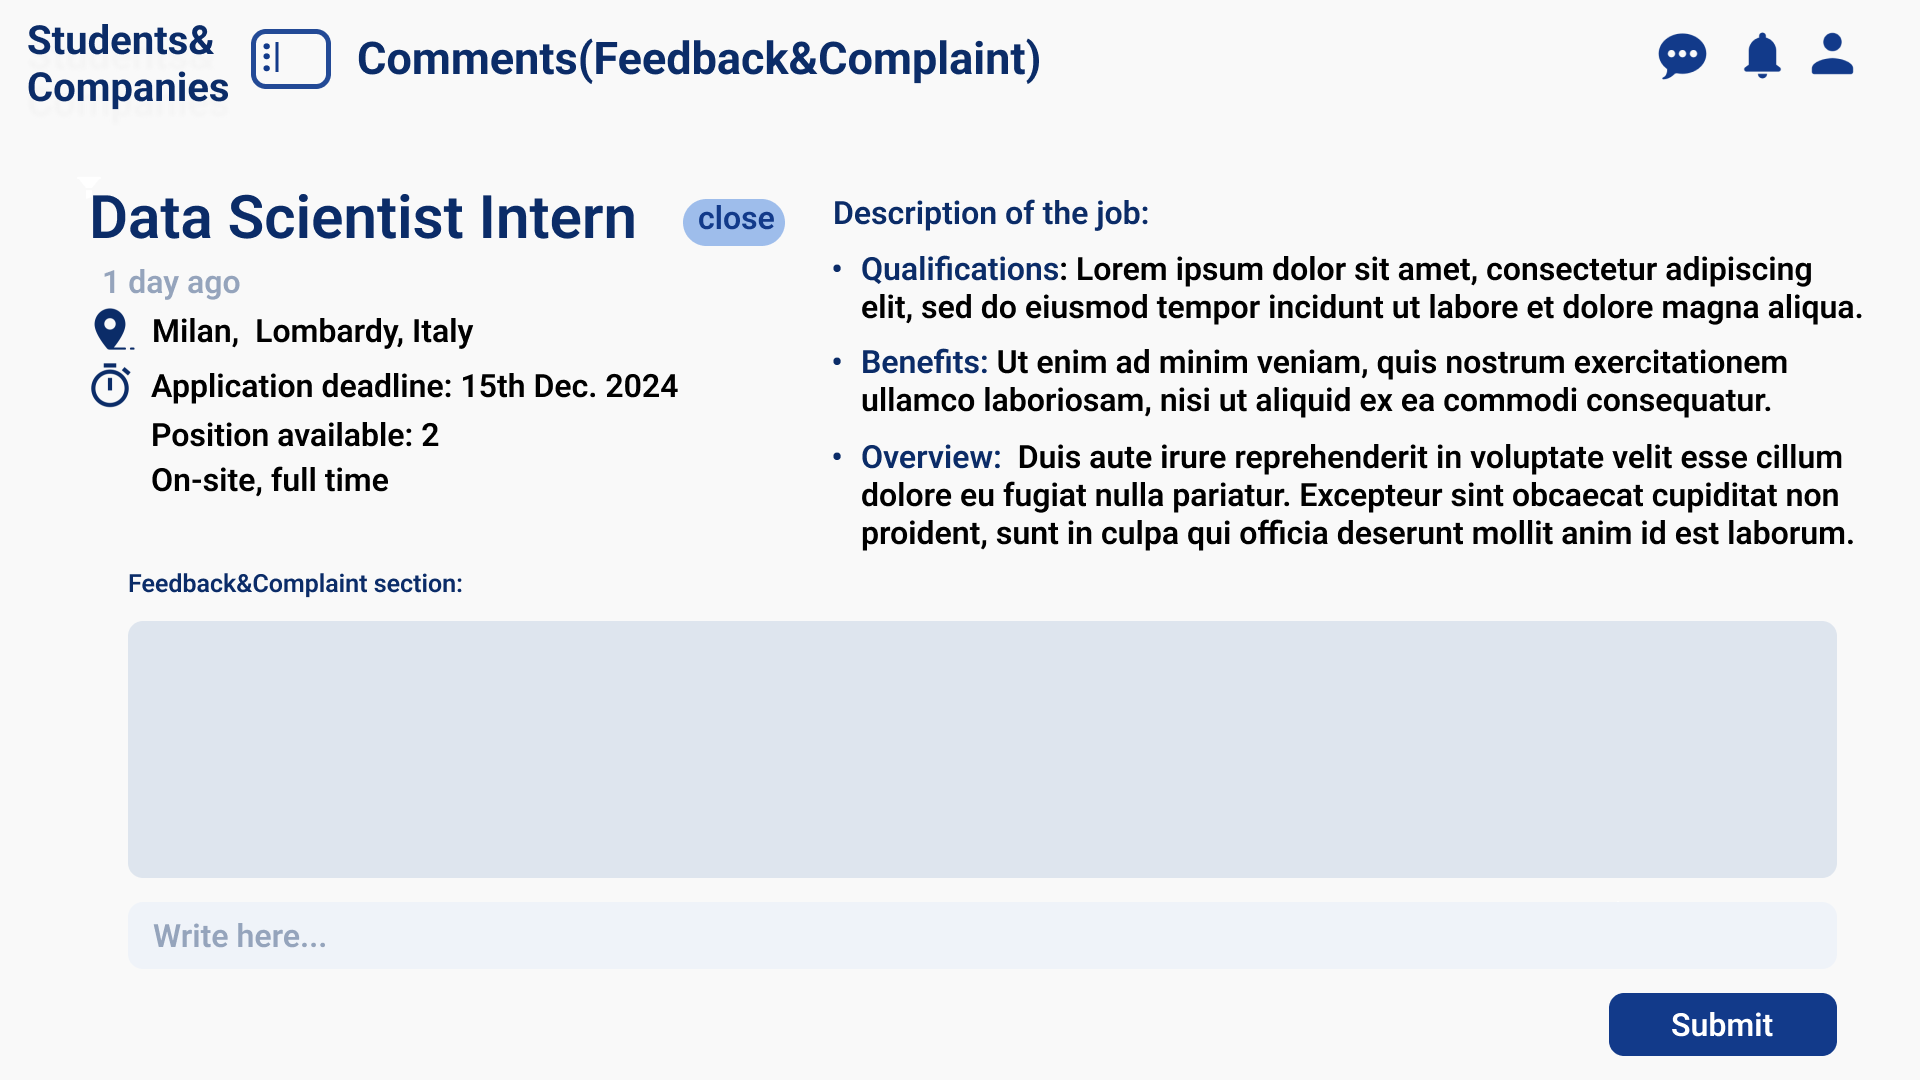
\includegraphics[width=0.8\textwidth]{Images/UI/FeedBack&Complaint- Student & Company.png}
    \caption{Feedback and Complaint}\label{fig:Feedback and Complaint}
\end{figure}

\newpage
\subsection{University's view}
For the university, the GUI is more simple than the student and company's view, because the university has only 
the role of monitoring the activities of its students.
As other users, the university can use the side menu to navigate to the desired page:
\textit{Search},\textit{Dashboard}.
\begin{figure}[H]
    \centering
    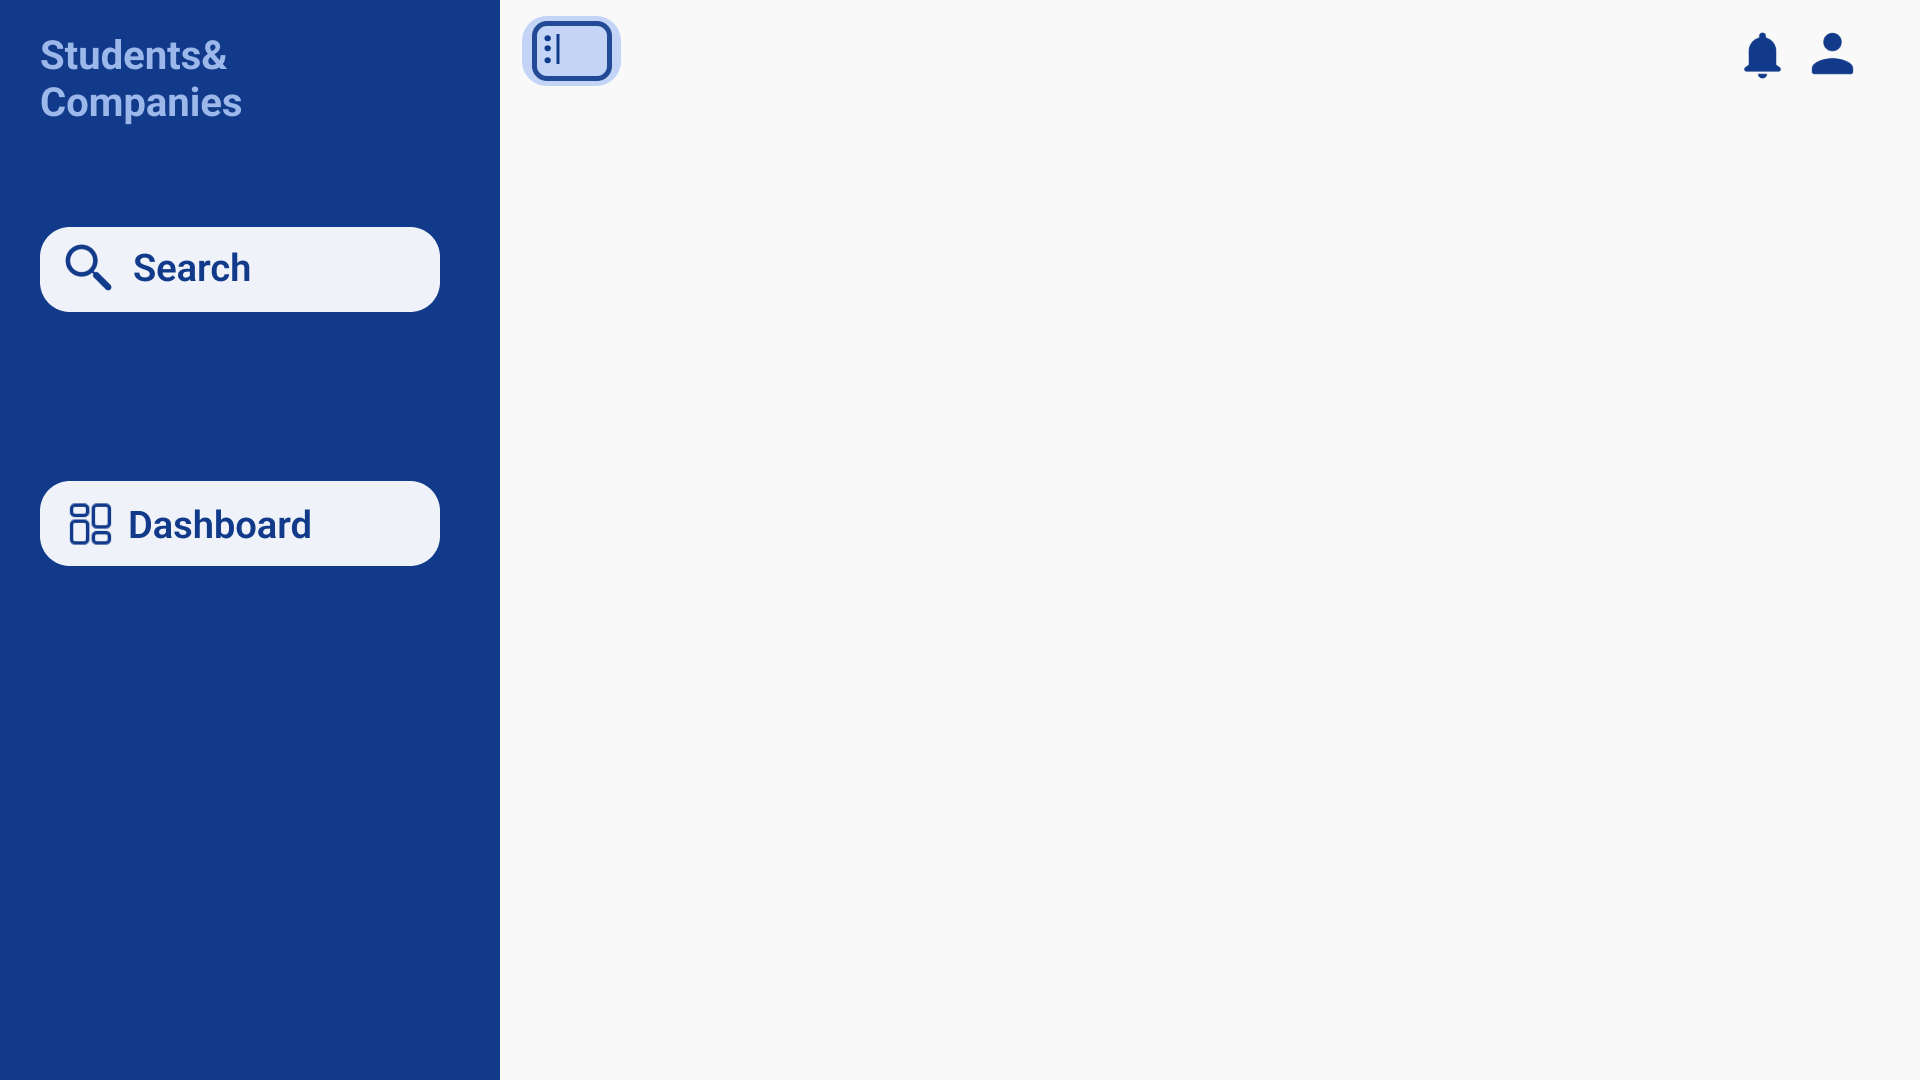
\includegraphics[width=0.8\textwidth]{Images/UI/Layout-University.png}
    \caption{University's Side Menu}\label{fig:University_view}
\end{figure}
\subsubsection{Dashboard page}
The university is directed to the Dashboard page upon logging in. The search bar, the Student list and a 
specific student's activities overview will be displayed in this page. To change the student, click on 
the box of certain student in the Student list, the student's activities overview will be updated and showed
respectively. If the university wants to view the Student's profile, click on the \textit{Profile details} button.
\begin{figure}[H]
    \centering
    \includegraphics[width=0.8\textwidth]{Images/UI/Dashboard 1-university.png}
    \caption{University's Dashboard 1}\label{fig:DashboardUniversity1}
\end{figure}

\subsubsection{FeedBack and Compalint page}
This page will be displayed when the university click on the \textit{View details} button of one of the student's activities.
The university can view the feedback and complaints history written by the student and the company during the internship and 
at the end of the internship.

\begin{figure}[H]
    \centering
    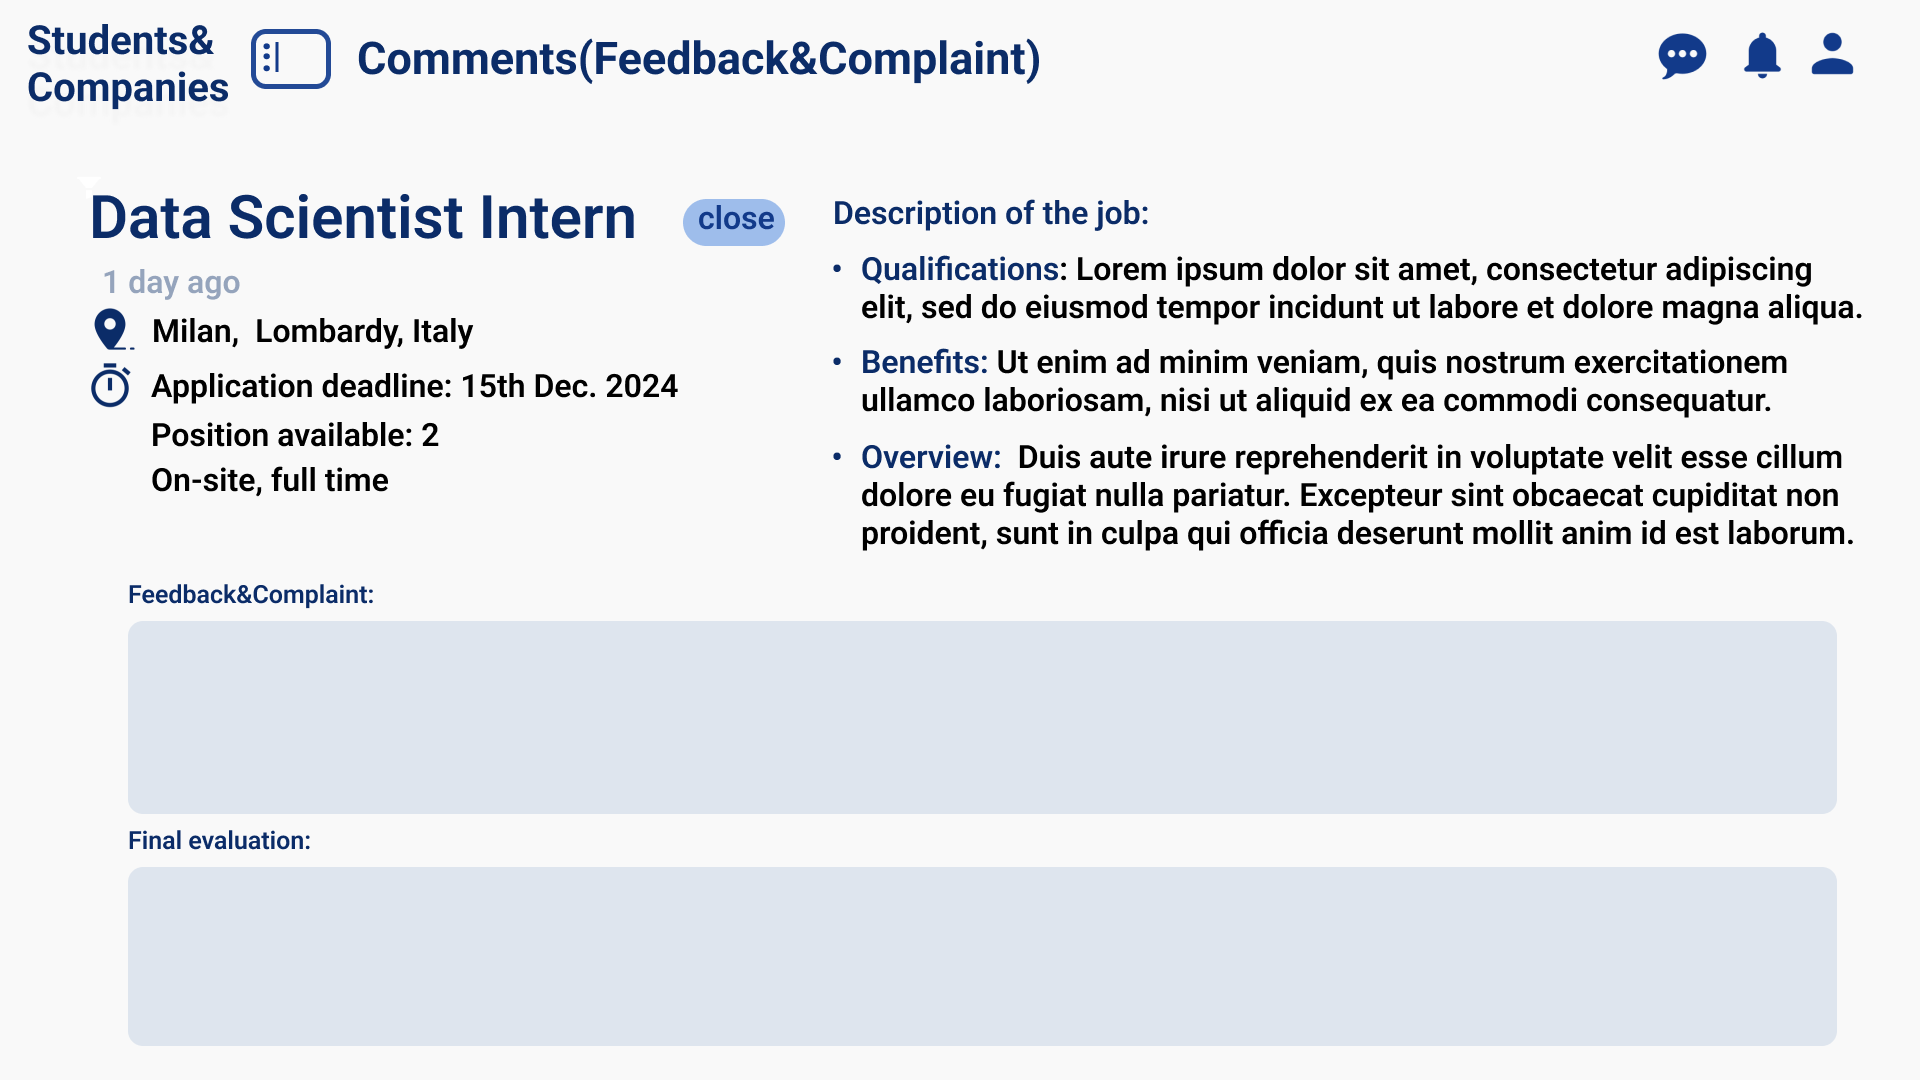
\includegraphics[width=0.8\textwidth]{Images/UI/FeedBack&Complaint- University view.png}
    \caption{Feedback and Complaint}\label{fig:Feedback and Complaint University}
\end{figure}